% Chapter 5

\chapter{Symmetries, topology and edge states } % Main chapter title

\label{Chapter5} % For referencing the chapter elsewhere, use \ref{Chapter5} 
\fancyhead[LO, RE]{Part II. \emph{Kitaev wires}}
\chead{Chapter 5. \emph{Symmetries, topology \& edge states}} % This is for the header on each page - perhaps a shortened title

%----------------------------------------------------------------------------------------
In this chapter we study the symmetries and topology of the Kitaev wires. In section \ref{sec.SymmetriesTRandPH} we define the time reversal, particle-hole and sublattice transformations. We further show that the system has an intrinsic particle-hole symmetry. In section \ref{sec.Topology10foldway} we use the transformations to formulate the topological classification dubbed the tenfold way. In section \ref{sec.2wirestimereversalsymmetries} we analyse the time reversal symmetries of the system. In turn the system is classified according to the tenfold way. In section \ref{sec.2wires_CSinv} we calculate the topological invariants of the system and discuss the presence of gapless Majorana edge states. In section \ref{sec.edgestatesandkramers} we study the edge states in more detail. Finally, in section \ref{sec.2wirestransitionqualitative} we formulate two possibilities for the $p$- to $s$-wave phase transition in a qualitative manner. 

\section{Time reversal, particle-hole and sublattice transformations}
\label{sec.SymmetriesTRandPH}
The mean field Hamiltonian is diagonal in momentum space. This means that it is translationally invariant along the $x$-axis. Specifically, the (unitary) translation operator is defined through: $\tau(x_0)\psi_{j,F}(x)\tau^\dagger (x_0) = \psi_{j,F}(x + x_0)$. In momentum space, we get $\tau(x_0) c_{j,k} \tau^\dagger(x_0) = \text{e}^{ikx_0}c_{j,k}$, as one might expect. Hence, terms like $c^\dagger_{j,k} c_{j,k}$ and $c_{i,k}c_{j,-k}$ are invariant under the translation. This means that $H_{FF}$ is invariant as well. Because of the translational invariance, we enforce that the time reversal, $T$, and particle-hole transformation, $C$, do not mix states with different positions. Specifically:
\begin{align}
T \Psi(x) T^{-1} &= U^\dagger_T \Psi(x), \hspace{0.5cm} TiT^{-1} = -i, \nonumber \\
C \Psi(x) C^{-1} &= (U^*_C)^\dagger (\Psi^\dagger(x))^t, \hspace{0.5cm} CiC^{-1} = i, 
\label{eq.TRandPH.realspace}
\end{align}
with $\Psi(x) = \begin{bmatrix} \psi_{1,F}(x) & \psi^\dagger_{1,F}(x) & \psi_{2,F}(x) & \psi^\dagger_{2,F}(x) \end{bmatrix}^t$, $t$ the transpose operation and $T$, $C$ the time reversal and particle-hole transformation respectively. The construction $(\Psi^\dagger(x))^t$ is to make the entries of $\Psi(x)$ daggered, but still have $\Psi(x)$ as a column vector. The trivial particle-hole transformation, i.e. $U_C = \mathbb{I}$, is thus $\psi_{j,F}(x) \to \psi^\dagger_{j,F}(x)$. $U_T$ and $U_C$ are $4\times 4$ matrices. Enforcing that the transformed operators are fermionic as well ensures these matrices to be unitary. The operation on $i$ specifies that time reversal is antiunitary and the particle-hole transformation is unitary. For specific transformations it is possible to have some physical intuition for these transformations. We emphasize however that they are formal constructions which enable us to classify Hamiltonians, as we shall later see. In momentum space this definition leads to:
\begin{equation}
T C_k T^{-1} = U^\dagger_T C_{-k}, \hspace{0.5cm} C C_k C^{-1} = (U^*_C)^\dagger (C^\dagger_{-k})^t,  
\label{eq.TRandPH.momentumspace}
\end{equation}
with $C_k = \begin{bmatrix} c_{1,k} & c^\dagger_{1,-k} & c_{2,k} & c^\dagger_{2,-k} \end{bmatrix}^t$. In momentum space, the trivial particle-hole transformation is $c_{j,k} \to c^\dagger_{j,-k}$. The trivial time reversal transformation is $c_{j,k} \to c_{j,-k}$. By inspecting the transformations $TH_{FF}T^{-1}$ and $CH_{FF}C^{-1}$, we get the following symmetry requirements:
\begin{align}
TH_{FF}T^{-1} = H_{FF} \Leftrightarrow U_T\mathcal{H}^*_{FF,-k} U^\dagger_T = + \mathcal{H}_{FF,+k}, \nonumber \\
CH_{FF}C^{-1} = H_{FF} \Leftrightarrow U_C\mathcal{H}^*_{FF,-k} U^\dagger_C = - \mathcal{H}_{FF,+k}. 
\label{eq.Symmetryrequirements}
\end{align}
This means that we can think of the second quantization transformations $T$ and $C$ in terms of first quantization antiunitary transformations $\mathcal{T} = U_TK$ and $\mathcal{C} = U_CK$, where $K$ is the complex conjugation operator. This is a general property of these transformation, not restricted to our specific system \cite{Ludwig.Topology, Chiu.Topology}. The Hamiltonian at hand is a so-called Bogoliubov$-$de Gennes (BdG) Hamiltonian. These BdG Hamiltonians in general have a particle-hole symmetry. The reason is that there is a redundancy in the matrix structure of the Hamiltonian. Explicitly, the structure contains a $4\times 4$ matrix, even though there are only two energy solutions for each $k$. Another way of putting this is that the two Nambu spinors, $C^\dagger_k$ and $C_k$ are not independent. We can transform one into the other by going to $-k$ and flipping the entries. The redundancy means that we can choose $C$ to have no effect on the Nambu spinor:
\begin{equation}
C C_k C^{-1} =  \sigma_0\otimes \tau_1 (C^\dagger_{-k})^t = \begin{bmatrix} 0 & 1 & 0 & 0 \\ 1 & 0 & 0 & 0 \\ 0 & 0 & 0 & 1 \\ 0 & 0 & 1 & 0 \end{bmatrix} \begin{bmatrix} c^\dagger_{1,-k} \\ c_{1,k} \\ c^\dagger_{2,-k} \\ c_{2,k} \end{bmatrix} = \begin{bmatrix} c_{1,k} \\ c^\dagger_{1,-k} \\ c_{2,k} \\ c^\dagger_{2,-k} \end{bmatrix} = C_k,
\end{equation}
with $\sigma_0$ the identity in wire space and $\tau_1$ the first Pauli matrix in particle-hole space. $\otimes$ is the direct product. This means that $H_{FF}$ is invariant under $C$. Since it stems from a redundancy in the \textit{structure} of the Hamiltonian, it is often referred to as a particle-hole \textit{constraint} of BdG systems rather than a symmetry.

By composing the time reversal and particle-hole transformations we can form a third transformation; the sublattice (or chiral) transformation $S = TC$. It is evident that this transformation is antiunitary like $T$. The same analysis as in the above leads to the symmetry condition:
\begin{equation}
SH_{FF}S^{-1} = H_{FF} \Leftrightarrow U_S\mathcal{H}_{FF,+k} U^\dagger_S = - \mathcal{H}_{FF,+k}.
\end{equation}
Hence, the transformation in first quantization is unitary, but has to \textit{anti}commute with the Hamiltonian. We explain the reason for studying these transformations in the next section.

\section{Topology and the tenfold way} \label{sec.Topology10foldway}
In the articles \cite{Ludwig.Topology, Chiu.Topology} it is studied, how one in the broadest possible sense can classify \textit{all} noninteracting fermionic Hamiltonians that has an energy gap in the spectrum. This includes insulators and superconductors. Hence, the authors build a framework in which two distinct Hamiltonians are viewed as equivalent, if one can continuously deform one to the other without closing the energy gap. These sort of deformations are linked to the study of topological spaces. Hence, the term \textit{topology}. Later we will see that the topology of the Hamiltonian has geometrical effects in real space, the edge states. However, as the above makes it clear, this is not the source of the term topology.  

One can use the three transformations of the previous section to classify the system within the above framework in the following manner. There are three possibilities for the time reversal and particle-hole symmetries. Either there is no symmetry, indicated by a $0$, or there is a symmetry and then the transformations can square to plus and minus the identity, indicated with $\pm 1$. The sublattice symmetry can either by absent, $0$, or present, $1$. Per construction, if there is both a time reversal, $T$, and a particle-hole symmetry, $C$, present, there is also a sublattice symmetry, $S = T C$. On the other hand, if only $T$ or $C$ is present of the two, there cannot be a sublattice symmetry. Else, we would be able to make the remaining symmetry by composition. However, in the case of no $T$ nor $C$ symmetry, there is still two possibilities for $S$: symmetry or no symmetry. This is the reason for including this last transformation. In total we then have $(3\cdot 3 - 1) + 2 = 10$ possibilities of combining the symmetries. It is therefore also referred to as the tenfold way. 

\begin{table}[!b]
\def\arraystretch{1.5}
\centering
\begin{tabular}{|l||r r r||c c c c|}
 \hline \diagbox[height=2em]{Cartan}{$d$}   	&  T &  C & S					& 0 			 & 1 			  				   & 2 			   	& 3 				\\ \hline 
 \hline A    									&  $0$ &  $0$ & $0$				& $\mathbb{Z}$ 	 & 0 			  				   & $\mathbb{Z}$   & 0   			 	\\
 \hline AIII 									&  $0$ &  $0$ & $\phantom{+}1$	& 0 			 & $\mathbb{Z}$   				   & 0 			   	& $\mathbb{Z}$    	\\
 \hline AI   									& $+1$ &  $0$ & $0$				& $\mathbb{Z}$ 	 & 0 			  				   & 0 			   	& 0 			    \\
 \hline \textcolor{red}{BDI}	       			& $+1$ & $+1$ & $1$ 			& $\mathbb{Z}_2$ & \textcolor{red}{$\mathbb{Z}$}   & 0 			   	& 0 			 	\\
 \hline \textcolor{red}{D}	       				&  $0$ & $+1$ & $0$ 			& $\mathbb{Z}_2$ & \textcolor{red}{$\mathbb{Z}_2$} & $\mathbb{Z}$   & 0 				\\
 \hline \textcolor{red}{DIII}	    			& $-1$ & $+1$ & $1$ 			& 0 			 & \textcolor{red}{$\mathbb{Z}_2$} & $\mathbb{Z}_2$ & $\mathbb{Z}$ 	 	\\
 \hline AII	       								& $-1$ &  $0$ & $0$ 			& $2\mathbb{Z}$  & 0 			  				   & $\mathbb{Z}_2$ & $\mathbb{Z}$  	\\
 \hline CII	       								& $-1$ & $-1$ & $1$ 			& 0 			 & $2\mathbb{Z}$  				   & 0 			   & $\mathbb{Z}_2$  	\\
 \hline C	       								&  $0$ & $-1$ & $0$ 			& 0 			 & 0 			  				   & $2\mathbb{Z}$  & 0  			 	\\
 \hline CI	       								& $+1$ & $-1$ & $1$				& 0 			 & 0 			  				   & 0 			   & $2\mathbb{Z}$   	\\
 \hline 
\end{tabular}
\caption{Periodic table of topological superconductors and insulators. Cartan is the ten so-called Cartan classes. $d$ is the spatial dimension. A 0-value for T,C and S indicates no symmetry. For T and C the sign indicates the sign of the square $T^2$ and $C^2$ for a symmetry present. $S=1$ indicates presence of a sublattice symmetry. The sets to the right indicates in what set of numbers the topological index should be found. The Cartan classes of interest are shown in red, along with the corresponding topological index in $d = 1$ dimension. }
\label{tab.PeriodicTableTISC}
\end{table}

Classifying the Hamiltonians in this framework puts the Hamiltonian in a so-called Cartan class. The information from the classification is that the topological index has to be found in a specific set of numbers. This set can for example be the integers, $\mathbb{Z}$. The result of the articles is then that if two ground states have different integers as their topological index, they cannot be deformed continously into each other. This means that the deformation from one to the other includes a closing of the energy gap. The so-called periodic table for topological insulators and superconductors is shown in table \ref{tab.PeriodicTableTISC}.

Using the above classification scheme we can formulate the bulk-boundary correspondence principle. For the sake of argument assume that we have a wire of particles with open ends in $d = 1$ dimension with $T^2 = C^2 = +\mathbb{I}$ and $S = 1$. Then the system belongs to Cartan class BDI, with a topological index in the integers, $\mathbb{Z}$. Assume that the system is topological with index $1$. The vacuum is topologically trivial, say with index $0$. Now imagine that we follow the spatial transition from the topological wire to the trivial vacuum. The index then has to jump from $1$ to $0$ at the boundary. This means that the bulk energy gap must close at the edges of the wire. In turn gapless states form at the edges. We have hereby connected a bulk effect, the topological index, to a boundary effect, the edge states. 

\section{Time reversal symmetries} \label{sec.2wirestimereversalsymmetries}
We will now analyse the time reversal symmetries of the system at hand. They come in two classes: one where the symmetry works in each wire independently and one which swaps particles between the wires. These time reversal symmetries are important both to classify the Hamiltonian according to the tenfold way and to understand certain aspects of the $p$- to $s$-wave phase transition, as we shall later see. 

\subsection{With separate wires} 
\label{subsec.TRseparatewires}
In this subsection we will show that the system has two time reversal symmetries which keep the wires separated. These both square to $+\mathbb{I}$.

There are two possibilities for this symmetry: 
\begin{equation}
T_1 \begin{bmatrix} c^\dagger_{1,k} \\ c^\dagger_{2,k} \end{bmatrix} T_1^{-1} = \eta\sigma_0 \begin{bmatrix} c^\dagger_{1,-k} \\ c^\dagger_{2,-k} \end{bmatrix} = \eta\begin{bmatrix} c^\dagger_{1,-k} \\ c^\dagger_{2,-k} \end{bmatrix}, \hspace{0.5cm} T_2 \begin{bmatrix} c^\dagger_{1,k} \\ c^\dagger_{2,k} \end{bmatrix} T_2^{-1} = \eta\sigma_3 \begin{bmatrix} c^\dagger_{1,-k} \\ c^\dagger_{2,-k} \end{bmatrix} = \eta\begin{bmatrix} c^\dagger_{1,-k} \\  - c^\dagger_{2,-k} \end{bmatrix}, \nonumber
\end{equation} 
with $\sigma_j$ the $j$'th Pauli matrix operating in wire space and $\eta$ some overall phase. Since $(\eta\sigma_0)(\eta\sigma_0)^* = \sigma_0^2 = + \mathbb{I}$ and $(\eta\sigma_3)(\eta\sigma_3)^* = \sigma_3^2 = + \mathbb{I}$, we get that both time reversal transformations square to $+\mathbb{I}$. We see that up to a phase, these transformations consist of sending a state in $k$ to a state in $-k$ \textit{without} swapping the wires. 

The question is now: under what circumstances is $T_1$ or $T_2$ a symmetry of the Hamiltonian? The problematic terms under these time reversal transformations are the pairing terms of the Hamiltonian: $\Delta^{11}_k c^\dagger_{1,k}c^\dagger_{1,-k}, \Delta^{22}_k c^\dagger_{2,k}c^\dagger_{2,-k}$ and $\Delta^{12}_kc^\dagger_{2,k}c^\dagger_{1,-k}$. We remember time reversal is antiunitary: $TiT^{-1} = -i$. For the first term, connected to $\Delta^{11}_k$, both $T_1$ and $T_2$ hereby give:
\begin{equation}
\Delta^{11}_k c^\dagger_{1,k}c^\dagger_{1,-k} \overset{T_j}{\to} \Delta^{11*}_k \left(\eta c^\dagger_{1,-k}\right)\left(\eta c^\dagger_{1,k}\right) = -\eta^2\Delta^{11}_k c^\dagger_{1,k}c^\dagger_{1,-k}, \nonumber
\end{equation}
since $\Delta^{11}_k$ is chosen real. Since the first and last expression must be identical for one of the symmetries to be obeyed, we need $\eta^2 = -1$. The transformation of the second term, connected to $\Delta^{22}_k$, yields the same result. The relevant terms containing $\Delta^{12}_k$ transform according to:
\begin{equation}
\sum_k \Delta^{12}_k c^\dagger_{2,k}c^\dagger_{1,-k} \overset{T_j}{\to} \sum_k \Delta^{12*}_k \left(\pm \eta c^\dagger_{2,-k}\right)\left( \eta c^\dagger_{1,k}\right) = \mp \sum_k \Delta^{12*}_{k} c^\dagger_{2,k}c^\dagger_{1,-k}. \nonumber
\end{equation}
The last equality is achieved by going from $k$ to $-k$ in the sum, using that $\Delta^{12}_k$ is even in $k$ and that $\eta^2 = -1$. This shows that both $\Delta^{12}_k$ real and imaginary realises a time reversal symmetry which does not exchange the wires. Further, these both square to $ + \mathbb{I}$.

\subsection{With wire exchange}
\label{subsec.TRwireexchange}
In this subsection we will show that we can construct two types of time reversal symmetries of the system which exchange the wires. One is obeyed if the interwire pairing is imaginary; this squares to $+\mathbb{I}$. The other is obeyed if the interwire pairing is real; this squares to $-\mathbb{I}$. We will further shortly discuss the particle-hole and sublattice symmetries, and finally how the symmetries of the preceding and current subsection puts the Hamiltonian in a specific symmetry class. 

We first define a time reversal operator which squares to $ + \mathbb{I}$ and interchanges the wires: 
\begin{equation}
T_+\begin{bmatrix} c^\dagger_{1,k} \\ c^\dagger_{2,k} \end{bmatrix} T_+^{-1} = \eta\sigma_1 \begin{bmatrix} c^\dagger_{1,-k} \\ c^\dagger_{2,-k} \end{bmatrix} = \eta\begin{bmatrix} c^\dagger_{2,-k} \\ c^\dagger_{1,-k} \end{bmatrix},\nonumber
\end{equation} 
with $\sigma_1$ the first Pauli matrix operating in wire space and $\eta$ some overall phase. Hence, under this time reversal transformation a fermion from wire 1 is transformed into a fermion in wire 2 and acquires the phase $\eta$. Since $(\eta\sigma_1)(\eta\sigma_1)^* = \sigma_1^2 = + \mathbb{I}$ we get, that $T_+$ squares to \textit{plus} the identity. Since $\varepsilon_{1,k} = \varepsilon_{2,k}$, the only problematic terms under time reversal are still the pairing terms: $\Delta^{11}_k c^\dagger_{1,k}c^\dagger_{1,-k}, \Delta^{22}_k c^\dagger_{2,k}c^\dagger_{2,-k}$ and $\Delta^{12}_kc^\dagger_{2,k}c^\dagger_{1,-k}$. The first term transform according to:
\begin{equation}
\Delta^{11}_k c^\dagger_{1,k}c^\dagger_{1,-k} \overset{T_+}{\to} \Delta^{11*}_k \left(\eta c^\dagger_{2,-k}\right)\left(\eta c^\dagger_{2,k}\right) = -\eta^2\Delta^{11}_k c^\dagger_{2,k}c^\dagger_{2,-k}. \nonumber
\end{equation}
Here we use that $\Delta^{11}_k$ is chosen to be real. This term should be identical to the original term connected to the product $c^\dagger_{2,k}c^\dagger_{2,-k}$: $\Delta^{22}_k c^\dagger_{2,k}c^\dagger_{2,-k}$. Since, we have chosen the intrawire pairings real and with an overall sign difference, we need $\eta^2 = 1$. Hence $\eta = \pm 1$ is required. The transformation of $\Delta^{22}_k c^\dagger_{2,k}c^\dagger_{2,-k}$ leads to the same result. Further:
\begin{equation}
\Delta^{12}_k c^\dagger_{2,k}c^\dagger_{1,-k} \overset{T_+}{\to} \Delta^{12*}_k \left(\eta c^\dagger_{1,-k}\right)\left( \eta c^\dagger_{2,k}\right) = -\eta^2 \Delta^{12*}_k c^\dagger_{2,k}c^\dagger_{1,-k} = - \Delta^{12*}_k c^\dagger_{2,k}c^\dagger_{1,-k}. \nonumber
\end{equation}
Hence, we need $\Delta^{12*}_k = - \Delta^{12}_k$; the interwire pairing must be imaginary to obey this time reversal symmetry.\footnote{Had we chosen the phases of the intrawire pairings differently we could ensure a time reversal symmetry by changing the overall phase acquired under $T_+$.} As described in section \ref{sec.SymmetriesTRandPH} we can convert the second quantized operator to one in first quantization:
\begin{equation}
\mathcal{T}_+ = \sigma_1\otimes \tau_0 \cdot K, 
\label{eq.2wiresTpluswireexchangefirstquantization}
\end{equation}
where $K$ is the complex conjugation operator and $\tau_i$ are the Pauli matrices operating in particle-hole space. Here we have chosen $\eta = 1$. The symmetry is then described by the fact that: $\mathcal{T}_+\mathcal{H}_{FF,k} = \mathcal{H}_{FF,-k}\mathcal{T}_+$.

We now define a time reversal operator that squares to $ - \mathbb{I}$ and interchanges the wires:
\begin{equation}
T_-\begin{bmatrix} c^\dagger_{1,k} \\ c^\dagger_{2,k} \end{bmatrix} T_-^{-1} = \eta\sigma_2 \begin{bmatrix} c^\dagger_{1,-k} \\ c^\dagger_{2,-k} \end{bmatrix} = -i\eta\begin{bmatrix} c^\dagger_{2,-k} \\ - c^\dagger_{1,-k} \end{bmatrix}.\nonumber
\end{equation} 
This transformation is different from $T_+$ in the sense that there is an overall sign difference in the transformation of the two types of fermions. Since $(\eta \sigma_2)(\eta \sigma_2)^* = \sigma_2\sigma_2^* = - \sigma_2^2 = - \mathbb{I}$, this time reversal operator squares to \textit{minus} the identity. Again we ask under what conditions this is a symmetry of the Hamiltonian. Looking at the same terms as before we firstly get:
\begin{equation}
\Delta^{11}_k c^\dagger_{1,k}c^\dagger_{1,-k} \overset{T_-}{\to} \Delta^{11*}_k \left(-i\eta c^\dagger_{2,-k}\right)\left(-i\eta c^\dagger_{2,k}\right) = \eta^2\Delta^{11}_k c^\dagger_{2,k}c^\dagger_{2,-k}. \nonumber
\end{equation}
This term should be identical to the original term connected to the product $c^\dagger_{2,k}c^\dagger_{2,-k}$: $\Delta^{22}_k c^\dagger_{2,k}c^\dagger_{2,-k} = -\Delta^{11}_k c^\dagger_{2,k}c^\dagger_{2,-k}$. Hence, we need $\eta = \pm i$. Further:
\begin{equation}
\Delta^{12}_k c^\dagger_{2,k}c^\dagger_{1,-k} \overset{T_-}{\to} \Delta^{12*}_k \left(i\eta c^\dagger_{1,-k}\right)\left(-i\eta c^\dagger_{2,k}\right) = -\eta^2 \Delta^{12*}_k c^\dagger_{2,k}c^\dagger_{1,-k} = \Delta^{12*}_k c^\dagger_{2,k}c^\dagger_{1,-k}. \nonumber
\end{equation}
So we need $\Delta^{12*}_k = \Delta^{12}_k$. Hence, the interwire pairing must be real to obey this time reversal symmetry. In first quantization we can express this time reversal operator as:
\begin{equation}
\mathcal{T}_- = i\sigma_2\otimes\tau_0 \cdot K, 
\label{eq.2wiresTminuswireexchangefirstquantization}
\end{equation}
where again $\sigma_i, \tau_i$ are Pauli matrices operating in wire and particle-hole space respectively. 

The analyses of these two subsections give us four possible sublattice symmetries in the case of an imaginary or real interwire pairing. For an imaginary interwire pairing $S_+ = T_+C$ and $S_1 = T_1C$ are both symmetries of the system. Both time reversal symmetries in this case square to plus the identity and the system unambigously belong to Cartan class BDI. For a real interwire pairing, the system both have a time reversal symmetry that squares to $+ \mathbb{I}$ and one that squares to $-\mathbb{I}$. This means that we can both put the Hamiltonian in the Cartan class BDI \textit{and} DIII. See table \ref{tab.PeriodicTableTISC} for the details. 

This may seem a little confusing. Should the Hamiltonian not belong to a specific class according to its symmetries? We emphasize that the Cartan classes are not distinct in this sense per se. Rather one should think of the classification in the following sense. For a real interwire pairing we can both put the Hamiltonian in class BDI and DIII, corresponding to $T^2 = +\mathbb{I}$ and $T^2=-\mathbb{I}$ respectively. This means that we can ask what ground states are topologically distinct, if we preserve just one of these symmetries. Hence, the system is characterized by having \textit{two} topological invariants in this case, one in $\mathbb{Z}$ and one in $\mathbb{Z}_2 = \{-1, 1\}$. 

\section{Chern-Simons invariants and winding number}
\label{sec.2wires_CSinv}
In the previous section we have shown that the ground state of the system can be characterized by an integer, the topological invariant. This integer belongs to $\mathbb{Z}_2$ or $\mathbb{Z}$ depending on whether the system obeys a time reversal symmetry with $T^2 = -\mathbb{I}$ or $T^2 = + \mathbb{I}$. However, we said nothing about how to calculate it. This is the aim of the current section.

For systems with a sublattice symmetry, $S$, in odd spatial dimensions the topological invariant can be calculated from the so-called Chern-Simons invariant \cite{Ryu.Topology}. In one spatial dimension the Chern-Simons invariant is defined as:
\begin{equation}
\text{CS}_1 = \frac{i}{2\pi}\int_{\text{BZ}}dk \; \tr\left[\mathcal{A}_k\right],
\label{eq.definition.CS1}
\end{equation}
where BZ is short for the first Brillouin zone, and $\mathcal{A}_k$ is the so-called Berry connection. In the literature the Chern-Simons invariant is also referred to as the (total) polarisation. This naming has a physical reasoning in electronic topological insulators, because it is actually a measure of the charge polarisation as a consequence of the edge states \cite{FuKane2006}. Since there are no charge carriers in our system, we will not use this naming. However, the Chern-Simons invariant is related very simply to a winding number, $w$, through: $w = 2\text{CS}_1$. The norm of the winding number counts the number of edge states, and so the invariant still has a clear physical interpretation \cite{Chiu.Topology}. By assumption the energy spectrum has an energy gap. If we set the zero point of energy in the middle of this gap, the states to negative energies, $\ket{e^{-}_{j,k}}$, are the occupied bands: 
\begin{equation}
\mathcal{A}^{ij}_k = \bra{e^{-}_{i,k}}\partial_k\ket{e^{-}_{j,k}}.
\end{equation}
For the double wire system the Berry connection is a $2\times 2$ matrix. For a single wire it is simply a scalar. We return to the form of the actual topological invariant in three cases: the single wire, the double wire with imaginary interwire pairing and the double wire with real interwire pairing. 

\subsection{Single wire: the winding number} \label{subsec.topologicalinvariant.singlewire}
In this subsection we digress to the single wire system. This will give us a good intuition for what the topological invariant actually is. Further, we use the formalism developed here when we analyse the extended Kitaev chain in a one-dimensional Bose gas in part III of this thesis. 

The Hamiltonian kernel for wire 1 only is given by: 
\begin{equation}
\mathcal{H}^{1}_{FF,k} = \begin{bmatrix} \varepsilon_k & \Delta^{11}_k \\ \Delta^{11}_k & -\varepsilon_k \end{bmatrix} = \mathbf{h}(k)\cdot\boldsymbol\tau,
\label{eq.singlewire.Hamiltoniankernel}
\end{equation}
with $\boldsymbol\tau = (\tau_1, \tau_2, \tau_3)$ containing the Pauli matrices in particle-hole space and $\mathbf{h}(k) = (\Delta^{11}_k, 0, \varepsilon_k)$. The Hamiltonian is still of the Bogoliubov-de-Gennes type, so it still has a built-in particle-hole symmetry that squares to $+\mathbb{I}$. It also has the time reversal symmetry of the uncoupled wires; $T_1$ of subsection \ref{subsec.TRseparatewires}. This also squares to $+\mathbb{I}$. This shows that the Kitaev (single) wire belong to Cartan class BDI. The corresponding topological index is thus to be found in the integers. 

For the single wire $T_1$ is expressed through the first quantization operator $\mathcal{T}_1 = U_TK$, with $U_T = i\tau_3$ and $K$ the complex conjugation operator. Hence, we have $\mathcal{T}_1\mathcal{H}^{1}_{FF,k}\mathcal{T}^{-1}_1 = \mathcal{H}^{1}_{FF,-k}$. Now consider a more general Hamiltonian kernel $\mathcal{H}^{1}_k = \mathbf{h}(k)\cdot\boldsymbol\tau$, but with the same imposed symmetries. We define the mapping $\hat{h}(k) = \frac{\mathbf{h}(k)}{|\mathbf{h}(k)|}$, with $E_k = |\mathbf{h}(k)|$ the energy dispersion. The time reversal symmetry then forces $h_y(k) = 0$. This means that the mapping $\hat{h}(k)$ is restricted to a circle in the xz-plane.\footnote{Had we chosen the phase of $\Delta^{11}_k$ differently, the time reversal symmetry would also be different. This would in turn impose a specific phase between $h_x$ and $h_y$. Again the mapping is restricted to a circle.} For $\mathcal{H}^{1}_{FF,k}$, $h_z(k) = \varepsilon_k$ is dominant for $k\to \pm \infty$ with respect to the pairing, $\Delta^{11}_k$. We are only considering perturbations to this Hamiltonian, so we still enforce this behaviour. This means that $\hat{h}(k = \pm \infty) = \hat{z}$. Therefore, $\hat{h}(k)$ maps an integer number of times around $\mathbf{h} = 0$ where $E_k = 0$. This integer is called the \textit{winding number}, $w$, of the mapping and is in fact the topological invariant. We clarify this in the following way. The winding number is an integer, so it cannot change from say $0$ to $1$ without the mapping $\hat{h}$ being ill-defined in-between. The only way for $\hat{h}$ to become ill-defined is if the energy gap closes. It is exactly this which characterizes a topological phase transition. Further, the mapping is well-defined as long as the symmetries of the system are obeyed. 

We now return to the system at hand. We have $h_z(k) = \varepsilon_k$ and $h_x(k) = \Delta^{11}_k$. If we let $\theta_k$ denote the angle of $\hat{h}(k)$ with the $z$-axis, the winding number is:
\begin{equation}
w = \frac{1}{2\pi}\oint d\theta_k.
\label{eq.definition.windingnumber}
\end{equation} 
The angle $\theta_k$ is given by: $\tan(\theta_k) = \frac{h_x(k)}{h_z(k)} = \frac{\Delta^{11}_k}{\varepsilon_k}$. In turn $\theta_k(c) = \arctan\left(\frac{\Delta^{11}_k}{\varepsilon_k}\right) + c$ for some constant $c$. Calculating $d\theta_k = dk \cdot \partial_k \theta_k$ then gives:
\begin{equation}
w = \frac{1}{2\pi}\int dk \frac{\varepsilon_k\partial_k\Delta^{11}_k - \Delta^{11}_k\partial_k\varepsilon_k}{\varepsilon^2_k + (\Delta^{11}_k)^2}.
\label{eq.windingnumber.Kitaevsinglewire}
\end{equation} 
In the beginning of this section we argued the topological invariant can be calculated from the Chern-Simons invariant. In the next subsections we will go into detail of how to do this, here we simply wish to come with an intuitive link to the winding number. If we calculate the Berry connection, $\mathcal{A}_k = \bra{e^{-}_{k}}\partial_k\ket{e^{-}_{k}}$, and in turn the Chern-Simons invariant of equation \eqref{eq.definition.CS1}, $\text{CS}_{1,1}$, we get exactly $w = 2\text{CS}_{1,1}$. Hence, we see that for the single wire, twice the Chern-Simons invariant is simply the winding of $\hat{h}$ around $\mathbf{h} = 0$. We can hereby very directly understand, why the Chern-Simons invariant is in fact a topological invariant, at least in this simpler single wire case. 

\begin{figure}
\center
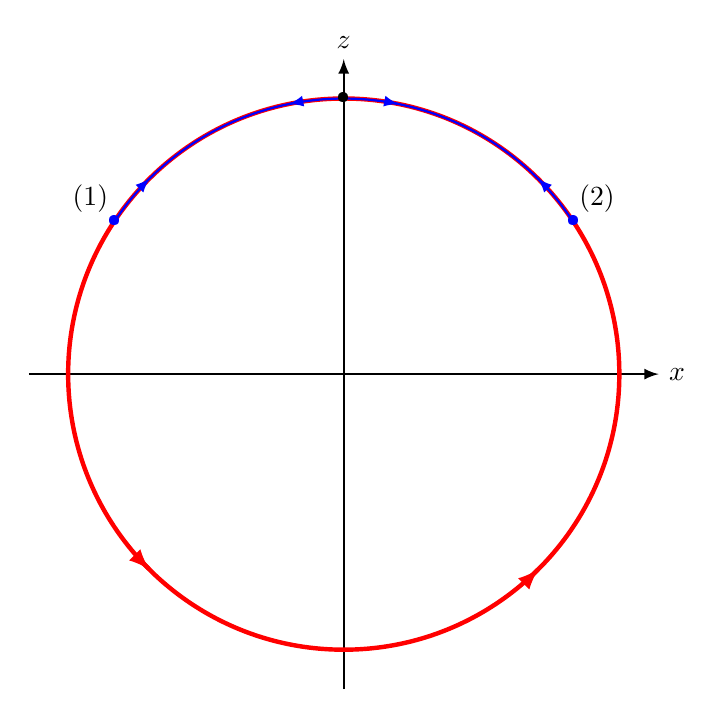
\begin{tikzpicture}
\draw[-latex, thick] ( 0.0, -4) -- (0, 4) node[above]{$z$};
\draw[-latex, thick] (-4,  0) -- (4, 0) node[right]{$x$};

\draw[red, ultra thick] (3.5, 0) arc (0:360:3.5);
\draw[-latex, red, ultra thick] (2.4648737348, -2.4848737348) -- (2.4748737348, - 2.4748737348);
\draw[-latex, red, ultra thick] (-2.4748737348, -2.4748737348) -- (-2.4648737348, -2.4848737348);

\draw[domain=33.540844097:146.459155903,smooth,variable=\x,blue, thick] plot ({3.5 * cos(\x)},{3.5 * sin(\x)});
\draw[-latex, blue, thick] (0.6853426578, 3.4322601227) -- (0.6953426578, 3.4302330223);
\draw[-latex, blue, thick] (2.4748737348,  2.4748737348) -- (2.4648737348, 2.4848737348);
\draw[-latex, blue, thick] (-0.6853426578, 3.4322601227) -- (-0.6953426578, 3.4302330223);
\draw[-latex, blue, thick] (-2.4748737348,  2.4748737348) -- (-2.4648737348, 2.4848737348);

%nodes:
\node[black] at (0, 3.5) {\textbullet};
\node[blue] at (-2.9172225397, 1.9338595227) {\textbullet};
\node[black] at (-2.9172225397 - 0.3, 1.9338595227 + 0.3) {(1)};
\node[blue] at (2.9172225397, 1.9338595227) {\textbullet};
\node[black] at (2.9172225397 + 0.3, 1.9338595227 + 0.3) {(2)};
\end{tikzpicture}
\caption{$\hat{h}(k)$ plotted parametrically as a function of $k$. The angle with respect to the $z$ axis is given by $\tan(\theta_k) = \Delta^{11}_k/\varepsilon_k$.  In blue: $\mu < 0$. The blue curve starts on the north pole, at the black dot. It then goes counterclockwise until it reaches the point (1). It turns around, goes clockwise until it reaches (2). Finally it returns to the north pole. The total winding number is $w = 0$. In red: $\mu > 0$. The red curve starts and ends at the north pole, at the black dot. It goes counterclockwise around 0. The total winding number is $w = -1$. }
\label{fig.hhatplot}
\end{figure}

From equation \eqref{eq.windingnumber.Kitaevsinglewire} it is clear that for vacuum, where $\Delta^{11}_k = 0$, the winding number is $w = 0$. Hence, this is the topologically trivial value. For nonzero pairing it turns out that there are three possibilities for the topological invariant: 
\begin{equation}
w = 2\text{CS}_{1,1} = \left\{ \begin{matrix} 
-\text{sgn}(\Delta^{11}_{k_0}) & \mu > 0, \\
0, & \mu < 0,
\end{matrix} \right. \nonumber 
\end{equation}
where $\text{sgn}$ denotes the sign function and $k_0 > 0$ is defined by $\varepsilon_{k_0} = 0$. In section \ref{subsec.2wires_CSinv_Delta12real} this result will appear as a limiting case to a more general result. The negative chemical potential case, $\mu < 0$, specifies a strong coupling phase, because the pairings strongly alters the chemical potential from the free gas one, $\epsilon_{F,0} > 0$. Here the system is topologically trivial: $w = 0$. In the same manner $\mu > 0$ specifies a weak coupling case with two possibilites, $w = \pm 1$, depending on the sign of the pairing, $\Delta^{11}_k$, at $k = k_0$. These are topologically nontrivial. This fits with the results for the Kitaev chain \cite{Alicea}. We have depicted the winding of $\hat{h}(k)$ in figure \ref{fig.hhatplot}. Here we assume $\Delta^{11}_k$ is negative for $k < 0$ and positive for $k > 0$. 

In the numerical analysis we will see that in the weak coupling limit we are investigating, the chemical potential is not significantly altered from the free gas Fermi energy, hence $\mu > 0$. Now suppose that the wire has open ends, with junctions to the vacuum with $\Delta^{11}_k = 0$. From equation \eqref{eq.windingnumber.Kitaevsinglewire} it is clear that the winding number is zero for vacuum: $w = 0$. The above topological analysis therefore shows that when we spatially follow the transition between the wire and vacuum, the winding number must jump from $w = \pm 1$ to $w = 0$ at the boundary. Therefore, the bulk gap goes to zero at the boundary. In turn an edge state with zero energy emerges. Now suppose that we introduce perturbations which respect the symmetries of the system. The robustness of the edge state can then be understood from the built-in particle-hole symmetry of the Hamiltonian. For the single wire the particle-hole symmetry is described by: $\mathcal{C} = \tau_1 K$, with $K$ the complex conjugation operator. Thus the perturbed Hamiltonian $\mathcal{H}_k$ obeys: $\mathcal{C}\mathcal{H}_{k} = -\mathcal{H}_{-k}\mathcal{C}$. Let us assume that we have a single particle energy solution in $k$: $\mathcal{H}_{k}\ket{\psi_k} = E_k\ket{\psi_k}$. We then get:
\begin{equation}
E_k\mathcal{C}\ket{\psi_k} = \mathcal{C}\mathcal{H}_{k}\ket{\psi_k} = -\mathcal{H}_{-k}\mathcal{C}\ket{\psi_k} \Rightarrow \mathcal{H}_{-k}\left(\mathcal{C}\ket{\psi_k}\right) = -E_k\left(\mathcal{C}\ket{\psi_k}\right).
\end{equation}
This shows that if $\ket{\psi_k}$ has the energy $E_k$, then $\mathcal{C}\ket{\psi_k}$ has the energy $-E_k$. In other words for every positive energy solution there is also a negative one, as is shown to the left in figure \ref{fig.edgestates}. The perturbations may move the bulk gap, $\Delta E$, because any low energy state with $E \neq 0 $ can simply be gapped away. This is indicated in the figure by the black dots and arrows. However, if the single gapless state at $E = 0$ moves either up or down, it breaks the +/- symmetry in the energies due to the built-in particle-hole symmetry. This leads to an energy spectrum which is \textit{robust} against symmetry-conserving perturbations. Here there is a continuum of states above the bulk gap and a \textit{single} zero energy edge state as indicated in figure \ref{fig.edgestates}. 

\begin{figure}
\center
\begin{tikzpicture}
\draw[|-latex, thick] (0, 0) -- (0,  2) node[above]{$E$};
\draw[-, thick]   (0, 0) -- (0, -2);
\node at (-0.4, 0) {$0$};

\draw[-, dashed] (0, 1)--(1, 1);
\draw[-, thick] (-0.1, 1)--(0.1, 1);
\node at (-1.17,1) {$\phantom{min[]}\Delta E$};

\draw[-, dashed] (0, -1)--(1, -1);
\draw[-, thick] (-0.1, -1)--(0.1, -1);
\node at (-1.38,-1) {$\phantom{min[]}-\Delta E$};

\draw[-, ultra thick] (1, 1)--(1, 2);
\draw[-, ultra thick] (1, -1)--(1, -2);
\node[red] at (1, 0) {\textbullet};

\node at (1, 0.5) {\textbullet};
\draw[-latex] (1, 0.5) --  (1,  1);
\node at (1, -0.5) {\textbullet};
\draw[-latex] (1, -0.5) -- (1, -1);

\draw[-, dashed] (0,0.01) --(1,0.01);

\draw[scale=0.5,domain=-1:1,smooth,variable=\x,red, thick] plot ({\x + 6},{ 3 * exp{- 10 * \x*\x}});
\draw[scale=0.5,domain=-1:1,smooth,variable=\x,red, thick] plot ({\x + 16},{ 3 * exp{- 10 * \x*\x}});

\node at (3, -0.4) {$0$};
\node at (8, -0.4) {$\mathcal{L}$};
\draw[|-latex, thick ] (3,0) -- (9,0) node[right]{$x$};

\draw[-, ultra thick ] (3,0) -- (8,0);
\end{tikzpicture}
\caption{To the left the energy spectrum is sketched. Because of the particle-hole symmetry, there is a negative energy state for every positive. $\Delta E$ is the bulk energy gap. There is a continuum of states above $\Delta E$ and below $-\Delta E$. Any low energy state can be perturbed away, but the particle-hole symmetry protects the single state at $E = 0$, indicated by the red dot. The corresponding wave function is sketched to the right.}
\label{fig.edgestates}
\end{figure}

\subsection{Double wire, imaginary interwire pairing} \label{subsec.2wires_CSinv_Delta12imag}
We now return to the double wire system. The results for the topological invariants are different for $\Delta^{12}$ real and imaginary. Therefore, they are treated separately. In this subsection we thus focus on calculating the $\mathbb{Z}$ topological invariant in the case of an imaginary interwire pairing. 

For an $\Delta^{12}$ imaginary, there is only a $T^2 = + \mathbb{I}$ symmetry. The topological invariant, $\nu_{\mathbb{Z}}$, is then given by the winding number, twice the Chern-Simons invariant:
\begin{align}
\nu_{\mathbb{Z}} &= 2\text{CS}_1 = \frac{i}{\pi} \int dk\; \text{tr}[\mathcal{A}] = \frac{i}{\pi} \int dk\; \left[\bra{e^{-}_{1,k}}\partial_k\ket{e^{-}_{1,k}} + \bra{e^{-}_{2,k}}\partial_k\ket{e^{-}_{2,k}}  \right] \nonumber \\
 &= 2(\text{CS}_{1,1} + \text{CS}_{1,2})\in \mathbb{Z}, \hspace{0.5cm} T^2 = +\mathbb{I}.
\label{eq.2wires.topinv.T2eqplus1}
\end{align}
Here we have indicated the contribution to the Chern-Simons invariant from the eigenvector $\ket{e^{-}_{i,k}}$ with $\text{CS}_{1,i}$. We will refer to these as the subsystem invariants. For $T^2 = +\mathbb{I}$ the subsystem invariants are not really topological invariants, only their sum is. In particular the subsystem invariants can take non-integer values in this case. 

We now calculate $\nu_{\mathbb{Z}}$. Since we differentiate the eigenvectors with respect to $k$, it is essential that these are well-behaved in any $k$. If we look closely at the eigenvectors derived back in section \ref{sec.HFFfull}, we can see that if $\Delta^{12}_k = 0$, the eigenvectors are not well-behaved in $k = 0$. Back then this was no issue, since a single problem point in the integral makes no difference.\footnote{One might be concerned about this line of thinking. However, the gap equations in the special cases investigated in the current section have also been derived using well-behaved eigenvectors. The result is the same.} Hence, the single truly tricky part is to get well-behaved eigenvectors. However, there is a procedure for it described in \cite{Ryu.Topology}. First we transform the Hamiltonian to the standard Nambu spinor form. Hence, we let $C_k \to \tilde{C}_k = \begin{bmatrix} c_{1,k} & c_{2,k} & c^\dagger_{1,-k} & c^\dagger_{2,-k}  \end{bmatrix}^{t}$. This amounts to the following transformation of $\mathcal{H}_{FF,k}$:
\begin{align}
\mathcal{H}_{FF,k} &= \varepsilon_k \sigma_0 \otimes \tau_3 + \Delta^{11}_k \sigma_3 \otimes \tau_1 + \Delta^{12}_k \sigma_2 \otimes \tau_1 \to \nonumber \\
\mathcal{H}'_{FF,k} &= \varepsilon_k \sigma_3 \otimes \tau_0 + \Delta^{11}_k \sigma_1 \otimes \tau_3 + \Delta^{12}_k \sigma_1 \otimes \tau_2,
\label{eq.Hamiltoniantostandardnambuspinorform} 
\end{align}
where $\otimes$ is the direct product and $\sigma_i, \tau_i$ are the Pauli matrices. We have also written the imaginary interwire pairing as $i\Delta^{12}_k$. Notice that we simply swap the indices of the $\tau$ and $\sigma$ matrices. Since the Hamiltonian both has a time reversal and particle-hole symmetry, it also has a sublattice symmetry anticommuting with the Hamiltonian in first quantization: $\{\mathcal{S}, \mathcal{H}_{FF,k}\} = 0$. In the new basis after the above transformation we see that $\mathcal{S} = \sigma_1\otimes \tau_1$. $\mathcal{S}$ has eigenvectors $v_{ab} = \chi^{1}_a\otimes \chi^{1}_b$, where $\chi^{1}_a$ for $a = 1,2$ are the eigenvectors to the first Pauli matrix $\tau_1, \sigma_1$. We then transform to the basis where $\mathcal{S}$ is diagonal by forming $V = (v_{ab})$ and calculating:
\begin{equation}
\tilde{\mathcal{H}}_{FF,k} = V^\dagger\mathcal{H}'_{FF,k}V = \varepsilon_k \sigma_1\otimes \tau_1 + \Delta^{11}_k \sigma_1\otimes\tau_3 - \Delta^{12}_k\sigma_2\otimes\tau_0. \nonumber 
\end{equation}
We then get the eigenvectors to negative energy eigenvalues:
\begin{equation}
\ket{e^{-}_{1,k}} = \frac{1}{2E_{F,k}}\begin{bmatrix} \varepsilon_k + i(\Delta^{11}_k + i\Delta^{12}_k) \\ i\left(\varepsilon_k + i\left(\Delta^{11}_k - i\Delta^{12}_k\right)\right) \\ -iE_{F,k} \\ -E_{F,k} \end{bmatrix}, \hspace{0.5cm} \ket{e^{-}_{2,k}} = \frac{1}{2E_{F,k}}\begin{bmatrix} \varepsilon_k + i(-\Delta^{11}_k - i\Delta^{12}_k) \\ -i\left(\varepsilon_k + i\left(-\Delta^{11}_k + i\Delta^{12}_k\right)\right) \\ iE_{F,k} \\ -E_{F,k} \end{bmatrix},
\end{equation}
with $E_{F,k} = \sqrt{\varepsilon_k^2 + (\Delta^{11}_k)^2 + (\Delta^{12}_k)^2}$. These eigenvectors are manifestly well-defined for all $k$. Using these we explicitly get:
\begin{equation}
\mathcal{A}^{11}_k = \bra{e^{-}_{1,k}}\partial_k\ket{e^{-}_{1,k}} = -\frac{i}{2E_{F,k}^2}(\Delta^{11}_k\partial_k\varepsilon_k - \varepsilon_k\partial_k\Delta^{11}_k) = -\mathcal{A}^{22}_k. \nonumber
\end{equation}
Hence, $\text{tr}[\mathcal{A}_k] = \mathcal{A}^{11}_k  + \mathcal{A}^{22}_k = 0$ and the topological invariant is simply $\nu_{\mathbb{Z}} = 0$. Since $\mathcal{A}^{11}_k$ vanishes for $\Delta^{11}_k = \Delta^{12}_k = 0$, $\nu_{\mathbb{Z}} = 0$ is the topologically trivial value. We conclude that the double wire system with $\Delta^{12}$ imaginary is topologically trivial. We will later see, what physical consequences this has by studying the edge states. We emphasize that the subsystem ``invariants'' given by $2\text{CS}_{1,j} = \frac{i}{\pi}\int dk \mathcal{A}^{jj}_k$ are not well-defined separately. In the present context it means they take non-integer values during the cross over, where both $\Delta^{11}_k$ and $\Delta^{12}_k$ are present. Only their sum, here equal to $0$, gives a topological invariant. Later we will numerically calculate these subsystem ``invariants''. From the above, they become:
\begin{equation}
\text{CS}_{1,1} = - \text{CS}_{1,2} = \frac{1}{4\pi}\int dk \; \frac{\Delta^{11}_k\partial_k\varepsilon_k - \varepsilon_k\partial_k\Delta^{11}_k}{\varepsilon^2_k + (\Delta^{11}_k)^2 + (\Delta^{12}_k)^2}. 
\end{equation}
These are continuous functions of $\Delta^{11}_k, \Delta^{12}_k$ and $\varepsilon_k$. Notice that for the uncoupled wires, $\Delta^{12}_k = 0$, we retrieve the winding number, $w$, for the single wire as discussed in the previous subsection. 


\subsection{Double wire, real interwire pairing} \label{subsec.2wires_CSinv_Delta12real}
In this subsection we calculate the topological invariants in the case of a real interwire pairing. 

For a real interwire pairing the system both has a $T^2 = +\mathbb{I}$ and $T^2 = -\mathbb{I}$ symmetry. The former is given by $T_2$ of section \ref{subsec.TRseparatewires} which only exchange particles within the same wire. The latter is given by $T_-$ of section \ref{subsec.TRwireexchange} which exchanges particles between the two wires. Therefore, the system both has $\mathbb{Z}$ and $\mathbb{Z}_2$ invariant. The $\mathbb{Z}$ invariant is given by equation \eqref{eq.2wires.topinv.T2eqplus1}.

The $\mathbb{Z}_2$ invariant is connected to the $T^2 = -\mathbb{I}$ symmetry. For such a time reversal symmetry, the states of the system come in time reversal, or Kramers, pairs. We will see this explicitly later on. At the present stage this means the subsystem invariants $\text{CS}_{1,i}$ of \eqref{eq.2wires.topinv.T2eqplus1} \textit{are} separately well-defined and it is meaningful to calculate their respective values \cite{FuKane2006, LiYangChen} and \cite[pp. 130-135]{BernevigTITSC}. The $\mathbb{Z}_2$ invariants can then be calculated by going to the so-called Wilson loop:
\begin{equation}
\nu_{\mathbb{Z}_2} = W_{1,j} = \text{e}^{2\pi i\text{CS}_{1,j}} = \pm 1, \hspace{0.5cm} T^2 = -\mathbb{I}.
\label{eq.2wires.topinv.T2eqminus1}
\end{equation}
We are now ready for the computation of the invariants. To get to well-behaved eigenvectors we follow the same procedure as outlined in the previous subsection. The $\Delta^{12}_k$ term of $\mathcal{H}_{FF,k}$ now has the form $\Delta^{12}_k \sigma_2 \otimes \tau_2$. After going to the Nambu spinor form, we therefore have $\mathcal{H}'_{FF,k} = \varepsilon_k \sigma_3 \otimes \tau_0 + \Delta^{11}_k \sigma_1 \otimes \tau_3 + \Delta^{12}_k \sigma_2 \otimes \tau_2$, recalling from equation \eqref{eq.Hamiltoniantostandardnambuspinorform} that we simply flip the indices of the $\tau$ and $\sigma$ matrices. The anticommuting sublattice symmetry is now given by: $\mathcal{S} = \sigma_1\otimes \tau_2$. The corresponding eigenvectors are therefore $v_{ab} = \chi^{1}_a\otimes\chi^{2}_b$, where again $\xi^{1}_a$ for $a = 1, 2$ are the eigenvectors to $\sigma_1$, etc. We let $V = (v_{ab})$ be the matrix of eigenvectors. In this basis $\mathcal{H}'_{FF,k}$ is:
\begin{equation}
\tilde{\mathcal{H}}_{FF,k} = V^\dagger\mathcal{H}'_{FF,k}V = \varepsilon_k \sigma_1\otimes \tau_1 + \Delta^{11}_k \sigma_1\otimes\tau_3 - \Delta^{12}_k\sigma_2\otimes\tau_1. \nonumber 
\end{equation}
The eigenvectors to negative eigenvalues, i.e. the occupied bands, are:
\begin{equation}
\ket{e^{-}_{1,k}} = \frac{1}{2E^{+}_{F,k}}\begin{bmatrix} \varepsilon_k + i(\Delta^{11}_k + \Delta^{12}_k) \\ i(\varepsilon_k + i(\Delta^{11}_k + \Delta^{12}_k)) \\ -iE^{+}_{F,k} \\ -E^{+}_{F,k} \end{bmatrix}, \hspace{0.5cm} \ket{e^{-}_{2,k}} = \frac{1}{2E^{-}_{F,k}}\begin{bmatrix} \varepsilon_k + i(-\Delta^{11}_k + \Delta^{12}_k) \\ -i(\varepsilon_k + i(-\Delta^{11}_k + \Delta^{12}_k)) \\ iE^{-}_{F,k} \\ -E^{-}_{F,k} \end{bmatrix}. \nonumber
\end{equation}
These are seen to be manifestly well-defined for all $k$. Notice that these eigenvectors are different from the ones for an imaginary interwire pairing, $\Delta^{12}_k$, in two ways. First, for a real interwire pairing the energies $E^{\pm}_{F,k}$ are in general different. Second, the front factors of $\Delta^{12}_k$ are altered. Since the entries of $\ket{e^{-}_{2,-k}}$ and $\ket{e^{-}_{1,+k}}$ are equal up to a sign, we get that:
\begin{equation}
\mathcal{A}^{11}_k = \bra{e^{-}_{1,k}}\partial_k\ket{e^{-}_{1,k}} = \bra{e^{-}_{2,-k}}\partial_k\ket{e^{-}_{2,-k}} = - \bra{e^{-}_{2,-k}}\partial_{-k}\ket{e^{-}_{2,-k}} = -\mathcal{A}^{22}_{-k}. \nonumber
\end{equation}
Hence, $\text{CS}_{1,2} = - \text{CS}_{1,1}$. The $\mathbb{Z}$ topological invariant is then trivial: $\nu_{\mathbb{Z}} = 2(\text{CS}_{1,1} + \text{CS}_{1,2}) = 0$. This is the same result as for imaginary $\Delta^{12}$, but remember that in this case $\text{CS}_{1,1}$ and $\text{CS}_{1,2}$ are individually conserved. The $\mathbb{Z}_2$ invariants are now calculated. First, we get:
\begin{equation}
\mathcal{A}^{11}_k = \bra{e^{-}_{1,k}}\partial_k\ket{e^{-}_{1,k}} = \frac{i}{2(E^{+}_{F,k})^2}\left(\varepsilon_k\partial_k(\Delta^{11}_k + \Delta^{12}_k) - (\Delta^{11}_k + \Delta^{12}_k)\partial_k \varepsilon_k\right) \nonumber
\end{equation}
The subsystem invariants are then:
\begin{equation}
\text{CS}_{1,1} = - \text{CS}_{1,2} = \frac{1}{4\pi}\int dk \; \frac{\varepsilon_k\partial_k(\Delta^{11}_k + \Delta^{12}_k) - (\Delta^{11}_k + \Delta^{12}_k)\partial_k \varepsilon_k}{\varepsilon_k^2 + (\Delta^{11}_k + \Delta^{12}_k)^2}.
\label{eq.CS11integralform}
\end{equation}
The integrand has a quite simple primitive:
\begin{equation}
\theta_k(c) = \arctan\left(\frac{\Delta^{11}_k + \Delta^{12}_k }{\varepsilon_k}\right) + c,
\label{eq.thetak.def}
\end{equation}
where $c$ is a constant. The evaluation of the integral itself however turns out to be a little subtle. There are two cases.

$\boldsymbol\mu \;\mathbf{< 0}$: $\varepsilon_k = \frac{k^2}{2m_F} - \mu$ is strictly positive for any $k$. This means that $\arctan\left(\frac{\Delta^{11}_k + \Delta^{12}_k }{\varepsilon_k}\right)$ is well-defined for all $k$ and we can use $\theta_k(c = 0)$ as the primitive. Then:
\begin{equation}
\text{CS}_{1,1} = \frac{1}{4\pi}\left.\arctan\left(\frac{\Delta^{11}_k + \Delta^{12}_k }{\varepsilon_k}\right)\right|^{\infty}_{-\infty} = 0, \nonumber
\end{equation}
as both $\Delta^{11}_k$ and $\Delta^{12}_k$ goes to $0$ and $\varepsilon_k \to \infty$ for $k\to \pm \infty$, and $\arctan(0) = 0$. This behaviour of the pairings is explicitly shown in the numerical analysis. Hence, for $\mu < 0$ we get $\nu = \text{e}^{2\pi i\text{CS}_{1,1}} = 1$ and the system is topologically trivial. 

$\boldsymbol\mu \; \mathbf{> 0}$: $\varepsilon_k$ has two zero points at the Fermi surface $k = \pm k_0$. This introduces discontinuities in $\theta_k(c = 0)$ at $\pm k_0$. However, for the evaluation of the integral to be correct, we must use a continuous primitive. Therefore we have to patch a continuous solution together by looking in the intervals $k < -k_0, -k_0 < k < +k_0$ and $k > +k_0$. Since $E^{\pm}_{F,k} = \sqrt{\varepsilon^2_k + |\Delta^{11}_k \pm \Delta^{12}_k|^2} \neq 0$ for all $k$ and $\varepsilon_{\pm k_0} = 0$, we get that $\Delta^{11}_{\pm k_0} + \Delta^{11}_{\pm k_0} \neq 0$. If this was not the case, the energy gap would close at either $+k_0$ or $-k_0$ and the topological index would be ill-defined, because the eigenvectors then becomes ill-defined at certain $k$-points. This means that $\text{sgn}(\Delta^{11}_k + \Delta^{12}_k)$ is well-defined in $k = \pm k_0$. By taking the limits around $\pm k_0$ of $\theta_k(c = 0)$ we can see that the following construction is a continuous primitive to the integrand in equation \eqref{eq.CS11integralform}:
\begin{equation}
\theta_k = \left\{ \begin{matrix} 
\arctan\left(\frac{\Delta^{11}_k + \Delta^{12}_k }{\varepsilon_k}\right) - \pi\text{sgn}(\Delta^{11}_{k_0} + \Delta^{12}_{k_0}), & k > k_0, \\
\arctan\left(\frac{\Delta^{11}_k + \Delta^{12}_k }{\varepsilon_k}\right), & -k_0 \leq k \leq k_0, \\
\arctan\left(\frac{\Delta^{11}_k + \Delta^{12}_k }{\varepsilon_k}\right) - \pi \text{sgn}(-\Delta^{11}_{k_0} + \Delta^{12}_{k_0}), & k < -k_0.
  \end{matrix} \right.
\label{eq.2wires.Gkmugreater0}
\end{equation}
We expect the pairings go to zero for $k\to \pm \infty$. We will verify this in the numerical analysis. Since $\varepsilon_k \overset{k\to \pm \infty}{\to} \infty$, the $\arctan$ part of $\theta_k$ goes to zero in these limits. Further, this means the signs $\text{sgn}(\Delta^{11}_{\pm k_0} + \Delta^{12}_{\pm k_0})$ must be different for $+$ and $-$ respectively for the integral to give a nonzero result. Since $\Delta^{12}_{k}$ is even and $\Delta^{11}_{k}$ is odd, this can only be achieved if $\Delta^{11}_{k}$ is dominant at the Fermi points: $|\Delta^{11}_{k_0}| > |\Delta^{12}_{k_0}|$. Hence, we get:
\begin{equation}
\text{CS}_{1,1} = \left. \frac{1}{4\pi} \theta_k \right|^\infty_{-\infty} = -\frac{1}{4}(\text{sgn}(\Delta^{11}_{k_0} + \Delta^{12}_{k_0}) - \text{sgn}(-\Delta^{11}_{k_0} + \Delta^{12}_{k_0})) = \left\{ \begin{matrix} 
-\frac{1}{2}\text{sgn}(\Delta^{11}_{k_0} + \Delta^{12}_{k_0}) , & |\Delta^{11}_{k_0}| > |\Delta^{12}_{k_0}|, \\
0, & |\Delta^{11}_{k_0}| < |\Delta^{12}_{k_0}|.
  \end{matrix} \right. \nonumber 
\end{equation}
This is the form we used for the winding number in subsection \ref{subsec.topologicalinvariant.singlewire} for $\Delta^{12}_k = 0$. The above results in the $\mathbb{Z}_2$ invariant:
\begin{equation}
\nu_{\mathbb{Z}_2} = \text{e}^{2\pi i \text{CS}_{1,1}} = \text{e}^{2\pi i \text{CS}_{1,2}} = \left\{ \begin{matrix} 
-1, & |\Delta^{11}_{k_0}| > |\Delta^{12}_{k_0}| & \text{and} & \mu > 0, \\
+1, & |\Delta^{11}_{k_0}| < |\Delta^{12}_{k_0}| & \text{or}  & \mu < 0.
  \end{matrix} \right.
\label{eq.CS11T2eqminus1}
\end{equation}
Hence, to be in a topological nontrivial phase we need to be in the weak coupling phase, $\mu > 0$. Further the intrawire pairing, $\Delta^{11}_k$, \textit{must} be dominant at the Fermi surface points $k = \pm k_0$, where $\varepsilon_{\pm k_0} = 0$. 

As a by-product of this subsection, we get that in the $d \to 0$ limit, the system is topologically trivial, since $\Delta^{12}_k$ is dominant here. This shows explicitly that a system with only $s$-wave pairing is topologically trivial. 

The combined result of the last two subsections is the following. If the interwire pairing, $\Delta^{12}$, is imaginary the double wire system is topologically trivial. If the interwire pairing is real, the system is topologically non-trivial, if the \textit{intra}wire pairing is dominant at the Fermi points and the chemical potential is positive. 

\section{Edge states and Kramers degeneracy} \label{sec.edgestatesandkramers}
In this section we will go into more detail with the edge states. We calculate approximate solutions for these in the case of uncoupled wires. We then go beyond mean field theory to address the question of how the interwire interaction influences these edge states. This is connected to Kramers degeneracy of time reversal partners.  

\subsection{Edge states: approximate solutions}
\label{subsec.2wiresedgestates}
We have now seen that a nonzero topological index leads to the existence of gapless edge states. Here we will explicitly show, how these edge states emerge for the uncoupled wires. The analysis is largely based on \cite[pp. 196-198]{BernevigTITSC}. 

\begin{figure}
\center
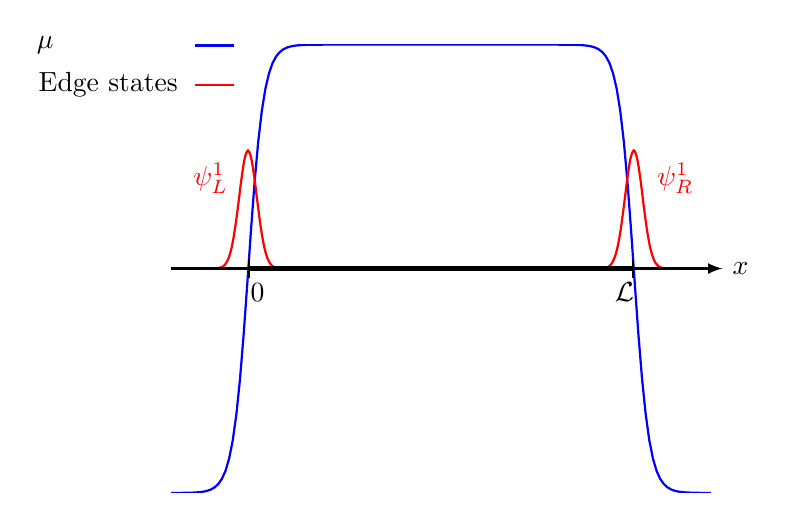
\begin{tikzpicture}
\begin{axis}[samples=150, xtick=\empty, ytick=\empty, axis line style={draw=none}, 
    xmin=-1, xmax=6,
    ymin = -1/2, ymax = 1/2,
    axis lines=center,
    domain=-1:6,
    ]

    \addplot [mark=none,draw=blue, thick] {1/2 * (tanh(5 * \x) - tanh(5 * (\x - 5) ) - 1)};
\end{axis}


\draw[scale=0.5,domain=-1:1,smooth,variable=\x,red, thick] plot ({\x + 0.975 * 2},{ 2 * 2.85 + 3 * exp{- 10 * \x*\x}});
\draw[scale=0.5,domain=-1:1,smooth,variable=\x,red, thick] plot ({\x + 5.875 * 2},{ 2 * 2.85 + 3 * exp{- 10 * \x*\x}});

\node at (0.975 + 0.12, 2.85 - 0.3) {$0$};
\node at (5.875-0.12, 2.85 - 0.3) {$\mathcal{L}$};
\draw[-latex, thick ] (0,2.85) -- (7,2.85) node[right]{$x$};
\draw[-, ultra thick ] (0.975,2.85) -- (5.875,2.85);
\draw[|-, thick ] (0.975,2.85) -- (1,2.85);
\draw[-, ultra thick ] (0.975,2.85) -- (5.875,2.85);
\draw[-|, thick ] (5.7,2.85) -- (5.875,2.85);

\coordinate (a) at (0.3, 5.682);
\coordinate (anode) at (-1.6, 5.682);
\coordinate (b) at (0.8, 5.682);
\coordinate (c) at (0.3, 5.182);
\coordinate (d) at (0.8, 5.182);
\coordinate (cnode) at (-0.8, 5.182);
\coordinate (wavefunctionnode11) at (0.5, 4.0);
\coordinate (wavefunctionnode12) at (6.4, 4.0);

\draw[-, thick, blue] (a) -- (b);
\node at (anode) {$\mu$}; 
\draw[-, thick, red] (c) -- (d);
\node at (cnode) {Edge states}; 
\node[red] at (wavefunctionnode11) {$\psi^{1}_{\text{L}}$};
\node[red] at (wavefunctionnode12) {$\psi^{1}_{\text{R}}$};
\end{tikzpicture}
\caption{Red: Edge states. Blue: chemical potential $\mu = \mu(x)$. Due to the spatial variation of the chemical potential the fermions are confined to the interval between $x = 0$ and $x = \mathcal{L}$. The uncoupled wires are topological for $\mu > 0$. For $\mu < 0$ they are trivial. Hence, edge states form around $\mu = 0$ at $x = 0$ and $x = \mathcal{L}$. Since the wires are uncoupled we only show wire 1.}
\label{fig.edgestatesmux}
\end{figure}

We would like to describe the Hamiltonian in real space, because we now ask whether certain states exist at the ends of the wires. To do this we define the operator $\Delta^{11}(p)$ as a function of the momentum operator $p = -i\partial_x$ in the following manner:
\begin{equation}
\Delta^{11}(p)\text{e}^{ikx} = \Delta^{11}_k\text{e}^{ikx}.
\label{eq.Deltapdef}
\end{equation}
Hence, we replace the variable dependency of $k$ in $\Delta^{11}_k$ with an operator dependency on $p$ in $\Delta^{11}(p)$. With this definition we get the Hamiltonian in real space:
\begin{equation}
H_{FF} = \frac{1}{2}\int dx\; \Psi^\dagger_{F}(x) \mathcal{H}_{FF}(x) \Psi_{F}(x), \hspace{0.5cm} \Psi_{F}(x) = \begin{bmatrix} \psi_{1,F}(x) & \psi^\dagger_{1,F}(x) & \psi_{2,F}(x) & \psi^\dagger_{2,F}(x)\end{bmatrix}^t
\label{eq.2wiresMFHamiltonianrealspace}
\end{equation}
With the real space Hamiltonian kernel:
\begin{equation}
\mathcal{H}_{FF}(x) = \begin{bmatrix} 
\frac{p^2}{2m_F} - \mu & \Delta^{11}(p) & 0 & 0 \\
\Delta^{11}(p) & -\left(\frac{p^2}{2m_F} - \mu \right) & 0 & 0 \\
0 & 0 & \frac{p^2}{2m_F} - \mu & -\Delta^{11}(p) \\
0 & 0 & -\Delta^{11}(p) & -\left(\frac{p^2}{2m_F} - \mu \right)
\end{bmatrix}.
\label{eq.2wiresMFHamiltonianrealspacefirstquantization}
\end{equation}
For the sake of clarity let us see how e.g. the term $\Delta^{11}_kc_{1,-k}c_{1,k}$ appears from this expression:
\begin{align}
\int dx \; \psi_{1,F}(x) \Delta^{11}(p) \psi_{1,F}(x) &= \frac{1}{\mathcal{L}}\sum_{k,q}c_{1,k} c_{1,q}\int dx \; \text{e}^{ikx}\Delta^{11}(p)\text{e}^{iqx} = \frac{1}{\mathcal{L}}\sum_{k,q}\Delta^{11}_qc_{1,k}c_{1,q}\int dx \; \text{e}^{i(k + q)x} \nonumber \\
&= \sum_{k}\Delta^{11}_kc_{1,-k}c_{1,k}, \nonumber 
\end{align}
since $\int dx\; \text{e}^{i(k + q)x} =\mathcal{L} \delta_{k,-q} $. Here we use the Fourier decomposition $\psi_{1,F}(x) = \frac{1}{\sqrt{L}}\sum_k\text{e}^{ikx}c_{1,k}$. Now we form junctions of topogically distinct phases by changing the sign of $\mu$ at $x = 0$ and $x = \mathcal{L}$. Hence, we let $\mu = \mu(x)$ as shown in figure \ref{fig.edgestatesmux}. Due to the spatial variation of the chemical potential the fermions are confined to the wire between $x = 0$ and $x = \mathcal{L}$. In first quantization we find solutions by solving $\mathcal{H}(x)\psi(x) = E\psi(x)$. The edge states are zero energy modes, so we solve for $E = 0$. We assume that $\mu(x)$ varies slowly over the interparticle length scale $1/k_F$. When this is fulfilled the solution $\psi(x)$ will also vary slowly and hence the curvature of $\psi(x)$ proportional to $p^2\psi(x)$ is negligible. This means that to a good approximation we only keep the operator $p$ up to first order. Since the intrawire pairing, $\Delta^{11}_k$, is $p$-wave type, it is linear in $k$ for $k/k_F \ll 1$. We will also verify this in the numerical analysis in chapter \ref{Chapter6}. This means that $\Delta^{11}(p)$ is linear in $p$, when $p/k_F$ used on a state is small. Hence, we ignore $p^2/2m_F$ and let $\Delta^{11}(p) = \Delta^{11} \cdot \tilde{p}$, with $\Delta^{11} = k_F\left.\frac{\partial \Delta^{11}_k}{\partial k}\right|_{k=0}$ and $\tilde{p} = p/k_F$. We assume $\Delta^{11} > 0$. We take the ansatz:
\begin{equation}
\psi^{i}_{\text{L}}(x) = \exp\left(-\frac{k_F}{\Delta^{11}}\int_{0}^{x} dx'\; \mu(x') \right)\mathbf{u}^{i}_{\text{L}}, \hspace{0.5cm} \psi^{i}_{\text{R}}(x) = \exp\left(+\frac{k_F}{\Delta^{11}}\int_{\mathcal{L}}^{x} dx'\; \mu(x') \right)\mathbf{u}^{i}_{\text{R}}, \nonumber
\end{equation}  
for four component vectors $\mathbf{u}^{i}_{\text{L,R}}$. The superscript ${}^i$ refers to the wire, the subscript ${}_{\text{L,R}}$ to which end the wave function is located, left and right respectively. Since $\Delta^{11}$ is in units of energy the exponents are unitless. Since $\Delta^{11} > 0$, we see that these states are exponentially localized at the edges. From this we get eigenvalue equations for $\mathbf{u}^{i}_{\text{L,R}}$. Defining $g_\text{L}(x) = \frac{1}{N}\text{e}^{-\frac{k_F}{\Delta^{11}}\int_{0}^{x} dx' \mu(x')}$, $g_\text{R}(x) = \frac{1}{N}\text{e}^{+\frac{k_F}{\Delta^{11}}\int_{\mathcal{L}}^{x} dx' \mu(x')}$ and $N^2 = \int dx |g_{\text{L,R}}(x)|^2$ a normalization constant we hereby get the approximate solutions:
\begin{align}
\psi^1_{\text{L}}(x) &= g_{\text{L}}(x)\frac{\text{e}^{+i\pi/4}}{\sqrt{2}}\begin{bmatrix} 1 & -i & 0 & 0 \end{bmatrix}^t , \hspace{0.5cm} \psi^1_{\text{R}}(x) = g_{\text{R}}(x)\frac{\text{e}^{-i\pi/4}}{\sqrt{2}}\begin{bmatrix} 1 & +i & 0 & 0 \end{bmatrix}^t, \nonumber \\
\psi^2_{\text{L}}(x) &= g_{\text{L}}(x)\frac{\text{e}^{-i\pi/4}}{\sqrt{2}}\begin{bmatrix} 0 & 0 & 1 & +i \end{bmatrix}^t , \hspace{0.5cm} \psi^2_{\text{R}}(x) = g_{\text{R}}(x)\frac{\text{e}^{+i\pi/4}}{\sqrt{2}}\begin{bmatrix} 0 & 0 & 1 & -i \end{bmatrix}^t.
\end{align}
These states solve $\mathcal{H}_{FF}\psi(x) = 0$. I.e. they have zero energy. They are the explicit forms of the gapless edge states. From equation \eqref{eq.2wiresTminuswireexchangefirstquantization} we have the time reversal operator that squares to minus the identity given by: $\mathcal{T}_- = i\sigma_2\otimes\tau_0 \cdot K$. Hence, $\mathcal{T}_-\psi^1_{\text{L}}(x) = -\psi^2_{\text{L}}(x)$ and $\mathcal{T}_-\psi^1_{\text{R}}(x) = -\psi^2_{\text{R}}(x)$. The edge states at the same end in each wire are therefore Kramers partners. This is crucial for the following analysis. For sake of completeness let us write up the second quantized version of the four states. The eigenstates define the diagonalisation matrix $U(x) = \begin{bmatrix} \psi^{1}_{1}(x) & \psi^{1}_{2}(x) & \psi^{2}_{1}(x) & \psi^{2}_{2}(x) \end{bmatrix}$. This has the unitarity property $\int dx \; U^\dagger(x) U(x) = \mathbb{I}$. We then let the operators $\gamma^{j}_{\text{L}}, \gamma^{j}_{\text{R}}$ for wire $j$ be given by:
\begin{equation}
\begin{bmatrix} \psi_{1,F}(x) \\ \psi_{1,F}^\dagger(x) \\ \psi_{2,F}(x) \\ \psi_{2,F}^\dagger(x) \end{bmatrix} = U(x) \begin{bmatrix} \gamma^{1}_{\text{L}} \\ \gamma^{1}_{\text{R}} \\ \gamma^{2}_{\text{L}} \\ \gamma^{2}_{\text{R}} \end{bmatrix} \Rightarrow \begin{bmatrix} \gamma^{1}_{\text{L}} \\ \gamma^{1}_{\text{R}} \\ \gamma^{2}_{\text{L}} \\ \gamma^{2}_{\text{R}} \end{bmatrix} = \int dx \; U^\dagger(x) \begin{bmatrix} \psi_{1,F}(x) \\ \psi_{1,F}^\dagger(x) \\ \psi_{2,F}(x) \\ \psi_{2,F}^\dagger(x) \end{bmatrix}.
\label{eq.Majoranaedgemodedef} 
\end{equation} 
Written out these operators are: 
\begin{align}
\gamma^1_{\text{L}} &= \int dx \; g_{\text{L}}(x)\frac{\text{e}^{-i\pi/4}}{\sqrt{2}}(\psi_{1,F}(x) + i\psi^\dagger_{1,F}(x)), \hspace{0.5cm} \gamma^1_{\text{R}} = \int dx \; g_{\text{R}}(x)\frac{\text{e}^{+i\pi/4}}{\sqrt{2}}(\psi_{1,F}(x) - i\psi^\dagger_{1,F}(x)), \nonumber \\
\gamma^2_{\text{L}} &= \int dx \; g_{\text{L}}(x)\frac{\text{e}^{+i\pi/4}}{\sqrt{2}}(\psi_{2,F}(x) - i\psi^\dagger_{2,F}(x)), \hspace{0.5cm} \gamma^2_{\text{R}} = \int dx \; g_{\text{R}}(x)\frac{\text{e}^{-i\pi/4}}{\sqrt{2}}(\psi_{2,F}(x) + i \psi^\dagger_{2,F}(x)). \nonumber 
\end{align}
In this manner $\psi^{i}_{\text{L,R}}(x)$ and $\gamma^{i}_{\text{L,R}}\ket{\text{S}}_0$ are equivalent. These operators are special in the sense that they are their own antiparticle: $\left(\gamma^{i}_{\text{L,R}}\right)^\dagger = \gamma^{i}_{\text{L,R}}$.\footnote{This also illuminates why we chose the rather arbitrary phase factors $\text{e}^{\pm i\pi/4}$. Had we \textit{not} done this, there would be some phase difference between $\left(\gamma^{i}_{\text{L,R}}\right)^\dagger$ and $\gamma^{i}_{\text{L,R}}$.} Such a fermionic particle is called a Majorana mode in condensed matter physics. Besides being their own antiparticle, they have to obey the modified anticommutator relation:
\begin{equation}
\{\gamma^{i_1}_{j_1}, \gamma^{i_2}_{j_2} \} = \delta_{i_1,i_2}\delta_{j_1,j_2}, \nonumber
\end{equation}
with $j_1, j_2 = \text{L}, \text{R}$. This is explicitly verified to be the case for the above operators.\footnote{Often one also meets the requirement that the anticommutator equals $2\delta_{i_1,i_2}\delta_{j_1,j_2}$. This is simply a matter of convention.} Since $(\gamma^{i}_{\text{L,R}})^\dagger \gamma^{i}_{\text{L,R}} = (\gamma^{i}_{\text{L,R}})^2 = 1/2$ we cannot count the Majorana edge states. In turn they do not represent physical states. We can remedy this by forming regular fermionic operators: $d_j = \frac{1}{\sqrt{2}}(\gamma^{j}_{\text{L}} + i\gamma^{j}_{\text{R}})$. The fermionic states described by these operators have equal weights in both end of each wire which can be separated by a macroscopic distance. By equal weights we mean that the probability of finding the states at the left end L is the same as finding them at the right end R.They are therefore highly non-local. This is also indicated in figure \ref{fig.edgestatesmux}. The chemical potential is linear around the left and right end. From this it follows that the wave functions are approximately gaussians, since they are $\propto \text{e}^{\pm \frac{k_F}{\Delta^{11}}\int dx\; \mu}$. 

The key result of this section is thus that $\ket{\text{S}}_0$ and $d_j^\dagger\ket{\text{S}}_0$ are degenerate ground states of the system. The latter topologically non-trivial state is therefore characterized by the presence of \textit{one} more particle than the former trivial one which is exponentially located on the edges. In second quantization the above notion of Kramers partners is described by the fact that: $T_-\gamma^1_{\text{L,R}}T_-^{-1} = \gamma^2_{\text{L,R}}$, simply because $\psi_{1,F}(x) \overset{T_-}{\to} \psi_{2,F}(x)$ and $T_-$ is antiunitary.

\subsection{Kramers degeneracy: protection of edge states}
\label{sec.2wireskramersdegeneracy}
Our analysis so far has been based on the mean-field BCS Hamiltonian. Here we want to go a little further and show that Kramers theorem protects the edge states in the two wires from becoming gapped by the interwire interaction, as long as it obeys the time reversal symmetry $T^2 = -\mathbb{I}$. 

Consider a general system described by the Hamiltonian $H$. Assume this Hamiltonian is time reversal invariant, $[T, H] = 0$, and that $T^2 = -\mathbb{I}$. Let $\ket{\psi_1}$ and $\ket{\psi_2}$ be eigenstates to the Hamiltonian, with energy $E_1$ and $E_2$, and Kramers partners: $\ket{\psi_2} = T\ket{\psi_1}$. Since $[T, H] = 0$ the two states have the same energy: 
\begin{equation}
E_2\ket{\psi_2} = HT\ket{\psi_1} = TH\ket{\psi_1} = E_1\ket{\psi_2}. \nonumber
\end{equation}
So $E_2 = E_1$. Further, the states are orthogonal:
\begin{equation}
\braket{\psi_1|\psi_2} = \braket{T\psi_2|T\psi_1} = \braket{-\psi_1|\psi_2} = -\braket{\psi_1|\psi_2} \Rightarrow \braket{\psi_1|\psi_2} = 0. \nonumber  
\end{equation}
In the first equality we use that we can flip the inner product by going to the time reversed states \cite[p. 274]{Sakurai}. In the second equality we use $T\ket{\psi_2} = -\ket{\psi_1}$, since $T^2 = -\mathbb{I}$. Hence, any energy state in a time reversal invariant system with $T^2 = -\mathbb{I}$ is twofold degenerate. This is Kramers degeneracy. Now let $H'$ be a perturbation to the Hamiltonian which respects the time reversal symmetry: $[T, H'] = 0$. In degenerate perturbation theory we calculate the matrix with entries $W_{ij} = \bra{\psi_i}H'\ket{\psi_j}$. The eigenstates of $H$ remain good eigenstates if the states uncouple: $\bra{\psi_1}H'\ket{\psi_2} = 0$: Equivalently $W_{ij}$ is diagonal. This is exactly the case for Kramers partners: 
\begin{equation}
\bra{\psi_1}H'\ket{\psi_2} = \bra{T\psi_2}TH'T^{-1}\ket{T\psi_1} = \bra{T\psi_2}H'\ket{T\psi_1} = -\bra{\psi_1}H'\ket{\psi_2} \Rightarrow \bra{\psi_1}H'\ket{\psi_2} = 0. \nonumber
\end{equation}
The first equality holds, since $H'$ is hermitian \cite[p. 274]{Sakurai}. 

Now what has this to do with the system at hand? We let $\ket{ \psi^{j}_{\text{L,R}} } = \gamma^{j}_{\text{L,R}}\ket{\text{S}}_0$ for wires $j = 1, 2$. In this way, $\ket{\psi^{1}_{\text{L}}}$ is the edge state in wire 1 at the left end, $\ket{\psi^{1}_{\text{R}}}$ in wire 1 at the right end, and so forth. From above we know that the edge states at end $i = L, R$, $\ket{\psi^1_{i}}$ and $\ket{\psi^2_{i}}$, are Kramers partners. If we can show that the interwire interaction $H' = H^\text{int,12}_{FF}$ is time reversal invariant under $T_-$, then the above analysis shows that the edge states at the same end of the two wires cannot couple. From equation \eqref{eq.Hint12realspace} we have:
\begin{equation}
H^\text{int,12}_{FF} = \int dx_1 dx_2 \psi^\dagger_{1,F}(x_1)\psi^\dagger_{2,F}(x_2) \tilde{V}_{\text{ind}}^{12}(x_1-x_2,0) \psi_{2,F}(x_2)\psi_{1,F}(x_1),
\end{equation}
with $\tilde{V}_{\text{ind}}^{12}(x_1-x_2,0)$ the zero frequency induced interaction in real space. Now $T_-\psi_{1,F}(x)T^{-1}_- = \psi_{2,F}(x)$ and $T_-\psi_{2,F}(x)T^{-1}_- = -\psi_{1,F}(x)$. Finally, $\tilde{V}_{\text{ind}}^{12}(x, 0)$ is real, so we get that $T_-H^\text{int,12}_{FF}T_-^{-1} = H^\text{int,12}_{FF}$. Hence, the edge states at the same end of the wire cannot couple. Further, the edge states at opposite ends of the wire are macroscopically separated. Therefore, these cannot couple either. In conclusion, the edge state in each wire is protected, as long as the interwire interaction is a perturbation to the system which is to say no interwire mean field has formed.  

\section{Qualitative understanding of cross over}
\label{sec.2wirestransitionqualitative}
In this section we come with a qualitative analysis of how the transition from $p$- to $s$-wave pairing as we tune the interwire distance, $d$, can occur using the previous two sections. 

$\mathbf{\Delta^{12}_k = 0}$: For the uncoupled wires the previous section shows that there is a single edge state in each wire. As the wires are brought closer together, the interwire interaction, $H^\text{int}_{FF,12}$, kicks in. Before any mean field of the interwire pairing has been chosen, the previous section further shows that the edge states stay uncoupled. This is the top of figure \ref{fig.2wiresedgestates}. 

\textbf{Imaginary interwire pairing}: Assume that as the wires are brought closer together, the system chooses the interwire pairing to be \textit{imaginary}. Then the system \textit{breaks} the time reversal symmetry $T_-$. In this case the protection of the edge states due to Kramers degeneracy as discussed in subsection \ref{sec.2wireskramersdegeneracy} is no longer present. As a consequence the edge states can couple and gap away. We can actually calculate by how much the edge states gap. In this connection we define the operator $\Delta^{12}(p)$ as: $\Delta^{12}(p)\text{e}^{ikx} = \Delta^{12}_k\text{e}^{ikx}$. Since $\Delta^{12}_k$ is even in $k$, there is no first order term in $k$. Hence for states with small curvatures like the edge states we can approximate $\Delta^{12}(p) = \Delta^{12}_{k=0}$, i.e. the operator reduces to a constant. Going back to the Hamiltonian kernel in momentum space, equation \eqref{eq.Hamiltoniankernelmomentumspace}, and treat the interwire pairing part as a perturbation, we see that the perturbation in real space relevant for the edge states is:
\begin{equation}
\mathcal{H}'_{FF}(x) = \Delta^{12}_{k=0}\begin{bmatrix} 
0 & 0 &  0 & -i \\
0 & 0 & -i & 0 \\
0 & i & 0  & 0 \\
i & 0 & 0  & 0  \end{bmatrix}
\label{eq.interwirepairingrealspace}
\end{equation}
The edge states in wires 1 and 2 in first quantization are described by the wave functions $\psi^1_{\text{L}}, \psi^2_{\text{L}}, \psi^1_{\text{R}}, \psi^2_{\text{R}}$ found in subsection \ref{subsec.2wiresedgestates} for wires $1$ and $2$. With this as an ordered basis we can calculate the perturbation matrix $W$ with entries $\bra{\psi^{i}_j}\mathcal{H}'\ket{\psi^{l}_k}$. We get:
\begin{equation}
W = \Delta^{12}_{k=0} \begin{bmatrix} 
0 & 0 & -i &  0 \\
0 & 0 &  0 & -i \\
i & 0 &  0 & 0 \\
0 & i &  0 & 0 \end{bmatrix} \nonumber
\end{equation}  
There are also couplings between the edge state at the left end in wire 1 with the edge state at the right end in wire 2 and vice versa. This coupling is proportional to the overlap of the wave functions $\int dx \; g_{\text{L}}(x)g_{\text{R}}(x)$ and is therefore exponentially suppressed by the length of the wire. Hence, it is negligible for a macroscopic system. In this sense the only nonzero couplings are between the edge states at the same end in each wire. The shift in energies are the eigenvalues of $W$. These along with the corresponding perturbed wave functions are then given by:
\begin{align}
E &= +\Delta^{12}_{k=0}, \hspace{0.5cm} \frac{1}{\sqrt{2}}\left( \psi^1_{\text{L,R}}(x) + i\psi^2_{\text{L,R}}(x) \right), \nonumber \\
E &= -\Delta^{12}_{k=0}, \hspace{0.5cm} \frac{1}{\sqrt{2}}\left( \psi^1_{\text{L,R}}(x) - i\psi^2_{\text{L,R}}(x) \right),
\label{eq.perturbededgestates}
\end{align}
for the edge at $x = 0$ and $x = \mathcal{L}$ indicated by $j = 1$ and $j = 2$ respectively. Hence, the interwire pairing couples the two edge states in each wire around $x = 0$ and the two edge states around $x = \mathcal{L}$. This makes it explicit, how the states are gapped! This is the content of figure \ref{fig.2wiresedgestates} going from the top center to the middle left. Note that it is only the states with positive energy which are physical. They are \textit{real} fermions as they consist of superpositions of two Majoranas.  

\textbf{Real interwire pairing}: Assume that as the wires are brought closer together, the system chooses the interwire pairing to be \textit{real}. In this situation the system still respects the time reversal symmetry, $T_-$. Kramers degeneracy is still present and therefore any energy state must be twofold degenerate. Further, since the system has a particle-hole symmetry the energy spectrum is symmetric around $E = 0$ (relative to the ground state). Therefore the zero energy edge states are locked as long as the bulk energy gap remains open. A direct calculation of the energy shift due to the coupling between the edge states by $\Delta^{12}$ performed in the same way as in the above verifies this explicitly. The bulk energy dispersions in this situation are given by: $E^{\pm}_{F,k} = \sqrt{\varepsilon^2_k + (\Delta^{11}_k \pm \Delta^{12}_k)^2}$. The bulk gap will therefore eventually close as we bring the wires closer together. This happens exactly when $|\Delta^{12}_{k_0}| = |\Delta^{11}_{k_0}|$, where $\pm k_0$ are the Fermi points given by: $\varepsilon_{\pm k_0} = 0$. It is therefore intuitively simple to see that in this case a topological phase transition takes place with a topologically non-trivial system for $|\Delta^{12}_{k_0}| < |\Delta^{11}_{k_0}|$ and a topologically trivial system for $|\Delta^{12}_{k_0}| > |\Delta^{11}_{k_0}|$, equation \eqref{eq.CS11T2eqminus1}. This is the content of figure \ref{fig.2wiresedgestates} going from the top center to the middle and bottom right. 

\begin{figure}
\center
\begin{tikzpicture}
\draw[|-latex, thick] (0, 0) -- (0,  2) node[above]{$E$};
\draw[-, thick]   (0, 0) -- (0, -2);
\node at (-0.4, 0) {$0$};

\draw[-, dashed] (0, 1)--(2, 1);
\draw[-, thick] (-0.1, 1)--(0.1, 1);
\node at (-0.7,1) {$E_{F,k_0}$};

\draw[-, dashed] (0,    -1) -- (2,   -1);
\draw[-, thick]  (-0.1, -1) -- (0.1, -1);
\node at (-0.85,-1) {$-E_{F,k_0}$};

\draw[-, ultra thick] (1, 1)--(1, 2);
\draw[-, ultra thick] (1, -1)--(1, -2);
\node[red] at (1, 0) {\textbullet};

\draw[-, ultra thick] (2, 1)--(2, 2);
\draw[-, ultra thick] (2, -1)--(2, -2);
\node[blue] at (2, 0) {\textbullet};

\draw[-, dashed] (0,0.01) -- (2,0.01);

\node at (3, -1.9) {$0$};
\node at (5, -1.9) {$\mathcal{L}$};

\draw[scale=0.5,domain=-1:1,smooth,variable=\x,red] plot ({\x + 6},{ 2 * exp{- 15 * \x*\x} - 3});
\draw[scale=0.5,domain=-1:1,smooth,variable=\x,red] plot ({\x + 10},{ 2 * exp{- 15 * \x*\x} -3});
\draw[|-latex, thick ] (3,-1.5) -- (5.8,-1.5) node[right]{$x$};
\draw[-, ultra thick ] (3,-1.5) -- (5,-1.5);

\node at (3, 1.1) {$0$};
\node at (5, 1.1) {$\mathcal{L}$};

\draw[scale=0.5,domain=-1:1,smooth,variable=\x,blue] plot ({\x + 6},{ 2 * exp{- 15 * \x*\x} + 3});
\draw[scale=0.5,domain=-1:1,smooth,variable=\x,blue] plot ({\x + 10},{ 2 * exp{- 15 * \x*\x} + 3});

\draw[|-latex, thick ] (3,1.5) -- (5.8,1.5) node[right]{$x$};
\draw[-, ultra thick] (3, 1.5) -- (5, 1.5);

%\draw[-, dashed] (5.8, -1.5) -- (5.8, 1.5);
\node at (2.2, 2.8) {$\Delta^{12}_k = 0$};

%%%%%%%%%%%%%%%%%%%%%%%%%%%%%%%%%%%
\pgfmathsetmacro{\hmove}{-4}
\pgfmathsetmacro{\vmove}{-6}

\draw[|-latex, thick] (\hmove, \vmove) -- (\hmove,  2 + \vmove) node[above]{$E$};
\draw[-, thick]   (\hmove, \vmove) -- (\hmove, -2 + \vmove);
\node at (-0.4 + \hmove, 0 + \vmove) {$0$};

\draw[-, dashed] (0 + \hmove, 1 + \vmove)--(2 + \hmove, 1 + \vmove);
\draw[-, thick] (-0.1 + \hmove, 1 + \vmove)--(0.1 + \hmove, 1 + \vmove);
\node at (-0.7 + \hmove, 1 + \vmove) {$E_{F,k_0}$};

\draw[-, dashed] (0 + \hmove,    -1 + \vmove) -- (2 + \hmove,   -1 + \vmove);
\draw[-, thick]  (-0.1 + \hmove, -1 + \vmove) -- (0.1 + \hmove, -1 + \vmove);
\node at (-0.85 + \hmove,-1 + \vmove) {$-E_{F,k_0}$};

\draw[-, ultra thick] (1 + \hmove, 1 + \vmove)--(1 + \hmove, 2 + \vmove);
\draw[-, ultra thick] (1 + \hmove, -1 + \vmove)--(1 + \hmove, -2 + \vmove);

%gapped edge state:
\coordinate (edge1energy) at (1 + \hmove, 0.5 + \vmove);
\node[right=0.0cm of edge1energy] {$+\Delta^{12}_{k=0}$}; 
\draw[-latex, semithick] (1 + \hmove, 0 + \vmove)--(1 + \hmove, 0.5 + \vmove);
\node[red] at (edge1energy) {\textbullet};

\draw[-, ultra thick] (2 + \hmove, 1 + \vmove)--(2 + \hmove, 2 + \vmove);
\draw[-, ultra thick] (2 + \hmove, -1 + \vmove)--(2 + \hmove, -2 + \vmove);

%gapped edge state:
\coordinate (edge2energy) at (2 + \hmove, -0.5 + \vmove);
\node[right=0.0cm of edge2energy] {$-\Delta^{12}_{k=0}$}; 
\draw[-latex, semithick] (2 + \hmove, 0 + \vmove)--(2 + \hmove, -0.5 + \vmove);
\node[blue] at (edge2energy) {\textbullet};

\draw[-, dashed] (0 + \hmove,0.01 + \vmove) -- (2 + \hmove,0.01 + \vmove);

\node at (3 + \hmove, -1.4 + \vmove) {$0$};
\node at (5 + \hmove, -1.4 + \vmove) {$\mathcal{L}$};

\draw[|-latex, thick ] (3 + \hmove,-1.0 + \vmove) -- (5.8 + \hmove,-1.0 + \vmove) node[right]{$x$};
\draw[-, ultra thick ] (3 + \hmove,-1.0 + \vmove) -- (5 + \hmove,-1.0 + \vmove);

\node at (3 + \hmove, 0.6 + \vmove) {$0$};
\node at (5 + \hmove, 0.6 + \vmove) {$\mathcal{L}$};

\draw[|-latex, thick ] (3 + \hmove, 1.0 + \vmove) -- (5.8 + \hmove,1.0 + \vmove) node[right]{$x$};
\draw[-, ultra thick] (3 + \hmove, 1.0 + \vmove) -- (5 + \hmove, 1.0 + \vmove);

\node at (2.2 + \hmove, 2.8 + \vmove) {$\Delta^{12}_k \neq 0$, imaginary};

%%%%%%%%%%%%%%%%%%%%%%%%%%%%%%%%%%%
\pgfmathsetmacro{\hmove}{4}
\pgfmathsetmacro{\vmove}{-6}
\pgfmathsetmacro{\Eminchange}{0.4}

\draw[|-latex, thick] (\hmove, \vmove) -- (\hmove,  2 + \vmove) node[above]{$E$};
\draw[-, thick]   (\hmove, \vmove) -- (\hmove, -2 + \vmove);
\node at (-0.4 + \hmove, 0 + \vmove) {$0$};

\draw[-, dashed] (0 + \hmove, 1 - \Eminchange + \vmove)--(2 + \hmove, 1 - \Eminchange + \vmove);
\draw[-, thick] (-0.1 + \hmove, 1 - \Eminchange + \vmove)--(0.1 + \hmove, 1 - \Eminchange + \vmove);
\node at (-0.7 + \hmove, 1 - \Eminchange + \vmove) {$E_{F,k_0}$};

\draw[-, dashed] (0 + \hmove,    -1 + \Eminchange + \vmove) -- (2 + \hmove,   -1 + \Eminchange + \vmove);
\draw[-, thick]  (-0.1 + \hmove, -1 + \Eminchange + \vmove) -- (0.1 + \hmove, -1 + \Eminchange + \vmove);
\node at (-0.85 + \hmove, -1 + \Eminchange + \vmove) {$-E_{F,k_0}$};

\draw[-, ultra thick] (1 + \hmove, 1 - \Eminchange + \vmove)--(1 + \hmove, 2 + \vmove);
\draw[-, ultra thick] (1 + \hmove, -1 + \Eminchange + \vmove)--(1 + \hmove, -2 + \vmove);
\node[red] at (1 + \hmove, 0 + \vmove) {\textbullet};

\draw[-, ultra thick] (2 + \hmove, 1 - \Eminchange + \vmove)--(2 + \hmove, 2 + \vmove);
\draw[-, ultra thick] (2 + \hmove, -1 + \Eminchange + \vmove)--(2 + \hmove, -2 + \vmove);
\node[blue] at (2 + \hmove, 0 + \vmove) {\textbullet};

\draw[-, dashed] (0 + \hmove, 0.01 + \vmove) -- (2 + \hmove, 0.01 + \vmove);

\node at (3 + \hmove, -1.4 + \vmove) {$0$};
\node at (5 + \hmove, -1.4 + \vmove) {$\mathcal{L}$};

\draw[scale=0.5,domain=-1:1,smooth,variable=\x,red] plot ({\x + 6 + 2*\hmove},{ 2 * exp{- 15 * \x*\x} - 2.0 + 2*\vmove});
\draw[scale=0.5,domain=-1:1,smooth,variable=\x,blue] plot ({\x + 10 + 2*\hmove},{ 2 * exp{- 15 * \x*\x} -2.0 + 2*\vmove});
\draw[|-latex, thick ] (3 + \hmove,-1.0 + \vmove) -- (5.8 + \hmove,-1.0 + \vmove) node[right]{$x$};
\draw[-, ultra thick ] (3 + \hmove,-1.0 + \vmove) -- (5 + \hmove,-1.0 + \vmove);

\node at (3 + \hmove, 0.6 + \vmove) {$0$};
\node at (5 + \hmove, 0.6 + \vmove) {$\mathcal{L}$};

\draw[scale=0.5,domain=-1:1,smooth,variable=\x,red] plot ({\x + 6  + 2*\hmove},{ 2 * exp{- 15 * \x*\x} + 2.0 + 2*\vmove});
\draw[scale=0.5,domain=-1:1,smooth,variable=\x,blue] plot ({\x + 10 + 2*\hmove},{ 2 * exp{- 15 * \x*\x} + 2.0 + 2*\vmove});

\draw[|-latex, thick ] (3 + \hmove,1.0 + \vmove) -- (5.8 + \hmove,1.0 + \vmove) node[right]{$x$};
\draw[-, ultra thick] (3 + \hmove, 1.0 + \vmove) -- (5 + \hmove, 1.0 + \vmove);

\node at (2.2 + \hmove, 2.8 + \vmove) {$|\Delta^{12}_{k_0}| < |\Delta^{11}_{k_0}|$, real};

%squezzing of gap:
\draw[-latex, semithick] (0.5 + \hmove, 1  + \vmove)--(0.5 + \hmove, 1 - \Eminchange + \vmove);
\draw[-latex, semithick] (0.5 + \hmove, -1 + \vmove)--(0.5 + \hmove, -1 + \Eminchange + \vmove);

%%%%%%%%%%%%%%%%%%%%%%%%%%%%%%%%%%%
\pgfmathsetmacro{\hmove}{4}
\pgfmathsetmacro{\vmove}{-12}
\pgfmathsetmacro{\Eminchange}{0.4}

\draw[|-latex, thick] (\hmove, \vmove) -- (\hmove,  2 + \vmove) node[above]{$E$};
\draw[-, thick]   (\hmove, \vmove) -- (\hmove, -2 + \vmove);
\node at (-0.4 + \hmove, 0 + \vmove) {$0$};

\draw[-, dashed] (0 + \hmove, 1 - \Eminchange + \vmove)--(2 + \hmove, 1 - \Eminchange + \vmove);
\draw[-, thick] (-0.1 + \hmove, 1 - \Eminchange + \vmove)--(0.1 + \hmove, 1 - \Eminchange + \vmove);
\node at (-0.7 + \hmove, 1 - \Eminchange + \vmove) {$E_{F,k_0}$};

\draw[-, dashed] (0 + \hmove,    -1 + \Eminchange + \vmove) -- (2 + \hmove,   -1 + \Eminchange + \vmove);
\draw[-, thick]  (-0.1 + \hmove, -1 + \Eminchange + \vmove) -- (0.1 + \hmove, -1 + \Eminchange + \vmove);
\node at (-0.85 + \hmove, -1 + \Eminchange + \vmove) {$-E_{F,k_0}$};

\draw[-, ultra thick] (1 + \hmove, 1 - \Eminchange + \vmove)--(1 + \hmove, 2 + \vmove);
\draw[-, ultra thick] (1 + \hmove, -1 + \Eminchange + \vmove)--(1 + \hmove, -2 + \vmove);
%\node[red] at (1 + \hmove, 0 + \vmove) {\textbullet};

\draw[-, ultra thick] (2 + \hmove, 1 - \Eminchange + \vmove)--(2 + \hmove, 2 + \vmove);
\draw[-, ultra thick] (2 + \hmove, -1 + \Eminchange + \vmove)--(2 + \hmove, -2 + \vmove);
%\node[blue] at (2 + \hmove, 0 + \vmove) {\textbullet};

\draw[-, dashed] (0 + \hmove, 0.01 + \vmove) -- (2 + \hmove, 0.01 + \vmove);

\node at (3 + \hmove, -0.9 + \vmove) {$0$};
\node at (5 + \hmove, -0.9 + \vmove) {$\mathcal{L}$};

\draw[|-latex, thick ] (3 + \hmove,-0.5 + \vmove) -- (5.8 + \hmove,-0.5 + \vmove) node[right]{$x$};
\draw[-, ultra thick ] (3 + \hmove,-0.5 + \vmove) -- (5 + \hmove,  -0.5 + \vmove);

\node at (3 + \hmove, 0.1 + \vmove) {$0$};
\node at (5 + \hmove, 0.1 + \vmove) {$\mathcal{L}$};

\draw[|-latex, thick ] (3 + \hmove,0.5 + \vmove) -- (5.8 + \hmove,0.5 + \vmove) node[right]{$x$};
\draw[-, ultra thick] (3 + \hmove, 0.5 + \vmove) -- (5 + \hmove,  0.5 + \vmove);

\node at (2.2 + \hmove, 2.8 + \vmove) {$|\Delta^{12}_{k_0}| > |\Delta^{11}_{k_0}|$, real};

%squezzing of gap:
\draw[-latex, semithick] (0.5 + \hmove, 1 - \Eminchange + \vmove)--(0.5 + \hmove, 1  + \vmove);
\draw[-latex, semithick] (0.5 + \hmove, -1 + \Eminchange + \vmove)--(0.5 + \hmove, -1 + \vmove);

\end{tikzpicture}
\caption{\textbf{Top centered}: for $\Delta^{12}_k=0$ we have two copies of the single wire system with the interwire interaction as a perturbation. There are two symmetry-protected edge states, one in each wire, and two energy dispersions mirrored in $E = 0$. The zero energy states are depicted as red and blue dots. The corresponding wave functions in red and blue as well. $k_0$ is defined by: $0 = \varepsilon_{k_0} = \frac{k^2_0}{2m_F} - \mu$. \textbf{Middle left}: If the system chooses an imaginary interwire pairing the system breaks the $T^2 = -\mathbb{I}$ symmetry. The edge states are therefore no longer protected at $E = 0$, and the edge states are gapped by $2\Delta^{12}_{k=0}$. \textbf{Middle and bottom right}: If the system chooses a real interwire pairing the system still respects the $T^2 = -\mathbb{I}$ symmetry. \textbf{Middle right}: Before an energy gap closing the edge states are still protected. Due to the interwire pairing the two edge states are located equally on each wire in opposite ends. Hence, the colours of the wave functions. The gap is closing; this is indicated by the arrows squezzing the gap. 
\textbf{Bottom right}: After the gap closing the edge states are gone. The system is topologically trivial. The gap is opening again indicated by the arrows.}
\label{fig.2wiresedgestates}
\end{figure}

It turns out that we can find the gapless eigenstates for $\Delta^{12}_{k=0} \ll \Delta^{11}$. We take the ansatz $\psi_{\text{L,R}}^{\pm}(x) = g_{\text{L,R}}^{\pm}(x)\cdot \mathbf{u}^{\pm}_{\text{L,R}}$ for four component vectors $\mathbf{u}^{\pm}_{\text{L,R}}$. Further $g_{\text{L}}^{\pm}(x) = \frac{1}{N}\text{e}^{-\frac{k_F}{\Delta^{11}}\int_0^x dx' \; \left[\mu(x') \pm i\Delta^{12}_{k=0}\right] }$ is located at the left end of the wires and $g_{\text{R}}^{\pm}(x) = \frac{1}{N}\text{e}^{+\frac{k_F}{\Delta^{11}}\int_{\mathcal{L}}^x dx' \; \left[\mu(x') \pm i\Delta^{12}_{k=0}\right] }$ is located at the right end of the wires. We then seach for solutions to $(\mathcal{H}_{FF}(x) + \mathcal{H}'_{FF}(x))\psi_{\text{L,R}}^{\pm}(x) = 0$, only keeping $p$ up to first order. The first and second derivative, $\partial^l_x$ for $l = 1, 2$, has a term proportional to $\left(\frac{\Delta^{12}_{k=0}}{\Delta^{11}}\right)^l\psi_j^{\pm}(x)$. Since we only keep $p$ up to first order, the second derivative must be small with respect to the first one. It is then clear that $\left(\frac{\Delta^{12}_{k=0}}{\Delta^{11}}\right)^2 \ll \frac{\Delta^{12}_{k=0}}{\Delta^{11}}$ is required. In turn $\Delta^{12}_{k=0} \ll \Delta^{11}$. As $\Delta^{12}_{k=0}$ comes closer to $\Delta^{11}$ we must add higher order terms in $p$ to get accurate results. With the above ansatz we get the following solutions in the $\Delta^{12}_{k=0} \ll \Delta^{11}$ regime:
\begin{align}
\psi_{\text{L}}^{+}(x) &= \frac{g_{\text{L}}^{+}(x)}{2}\begin{bmatrix} 1 & -i & 1 & i \end{bmatrix}^t, \hspace{0.5cm} \psi_{\text{R}}^{+}(x) = \frac{g_{\text{R}}^{+}(x)}{2}\begin{bmatrix} 1 & i & -1 & i \end{bmatrix}^t, \nonumber \\
\psi_{\text{L}}^{-}(x) &= \frac{g_{\text{L}}^{-}(x)}{2}\begin{bmatrix} i & 1 & -i & 1 \end{bmatrix}^t, \hspace{0.5cm} \psi_{\text{R}}^{-}(x) = \frac{g_{\text{R}}^{-}(x)}{2}\begin{bmatrix} -i & 1 & -i & -1 \end{bmatrix}^t.
\label{eq.zeromodesDelta12real}
\end{align}
This gives the explicit forms for the gapless Majorana modes in the presence of a real interwire pairing. From these solutions, we can form two real fermionic states with zero energy. The two first components of the vectors in the above expressions are the parts of the wave functions in wire 1, the last two components the parts of the wave functions in wire 2. It is therefore evident that the new edge states are localised with even probability in each wire due to the real interwire pairing. One is localised around $x = 0$, the other around $x = \mathcal{L}$ which is evident from the functions $g_{\text{L,R}}^{\pm}(x)$. This is indicated in the middle right of figure \ref{fig.2wiresedgestates} by the colours of the wave functions. Further, to lowest order in $\Delta^{12}_{k = 0}/\Delta^{11}$ the edge state wave functions simply acquire a space dependent phase proportional to $\Delta^{12}_{k=0}$.  

